\documentclass[a4paper,11pt]{article}

\usepackage{amsmath}
\usepackage{graphicx}
\usepackage[usenames, dvipsnames]{xcolor}
\usepackage[numbers, comma, sort&compress, super]{natbib}
\usepackage[english]{babel}
\usepackage[utf8]{inputenc}
\usepackage{lineno}
\usepackage{setspace}
\usepackage{verbatim}
\usepackage{lmodern}
\usepackage{microtype}
\usepackage[bf]{caption}
\usepackage{subcaption}
\usepackage[pdfborder={0 0 0}]{hyperref}
\usepackage[a4paper, left=25mm, right=25mm, top=30mm, bottom=30mm]{geometry}
\usepackage[small]{titlesec}
\usepackage{fancyhdr}

\newcommand{\ud}{\text{d}}
\newcommand{\dt}[1]{\frac{\ud #1}{\ud t}}
\newcommand{\ol}[1]{\overline{#1}}
\newcommand{\rem}[1]{\textcolor{red}{#1}}
\newcommand{\SI}{SI}
\newcommand{\MM}{Methods}
\let\originalleft\left
\let\originalright\right
\renewcommand{\left}{\mathopen{}\mathclose\bgroup\originalleft}
\renewcommand{\right}{\aftergroup\egroup\originalright}
%\hypersetup{colorlinks=true, urlcolor=blue}

\setlength{\headheight}{15pt}
\setlength{\parskip}{2ex}
\setlength{\parindent}{0.0ex}
\hyphenpenalty=10000
\clubpenalty=10000
\widowpenalty=10000
\tolerance=10000

\title{Vulnerability in the Serengeti food web - approximated with Bayesian Networks}
\author{Anna {\AA}kesson\\
\it \footnotesize University of Linkoping, Sweden\\
\it \footnotesize anna.akesson@liu.se}
\date{}

\begin{document}

\maketitle				
\onehalfspacing

\section*{Introduction}

Anthropogenic activities have significantly altered nature across the globe, with profound effects on both ecosystem functioning and on biodiversity, the latter declining at an unprecedented pace \cite{Diazetal2019}. Multiple factors connected to human activities are involved in the current and expected loss of species. One important factor is altered weather conditions following climate change - a factor considered to be one of the main drivers of species loss \cite{Zedan2004}. For example, global mean temperatures and mean precipitation, as well as precipitation extremes (causing both floods and droughts), are expected to increase \cite{IPCC}. Other important stressors are extensive land use causing habitat alteration and destruction \cite{Diazetal2019, Zedan2004}, as well as invasive species causing altered species compositions, habitat degradation and ultimately species loss \cite{Didhametal2005, MainkaHoward2010}. The loss of species does not only raise ethical concerns, but do alone affect ecosystem functioning and productivity to a magnitude comparable to many other global environmental changes \cite{Hooperetal2012}, making biodiversity loss an important stressor in itself. This cumbersome situation is a simple consequence of the nature of an ecological network. The loss of a species is not an isolated incident, and the extinction of a single species could potentially set in motion a cascade of secondary extinctions pertubating through the community by bottom-up effects \cite{EbenmanJonsson2005}. Primary producers, the basal level of an ecological network, are of great importance and the foundation of a community; plants connect to herbivores which connect to predators, and together they form an ecological network. ADD - primary producers are the first ones to be affected by changes, since they commonly respond fast to changes, and alterations in their composition potentially alter the complete ecological environment. Example, kelp forests but do also find examples on land. 

Policy makers and experts need effective methods to forecast extinction risk of species in order to take well-informed conservation decisions and resulting actions, if we are to mitigate the devastating effect of anthropogenic activities on biodiversity. Using Bayesian networks \cite{Jensen1996}, it is possible to estimate the extinction probability for each and every species present in an ecological network \citep{Eklofetal2013}. This method benefits from fast execution, a minimum of parameters necessary to estimate and easily interpreted results. Ekl\"{o}f et al. \citep{Eklofetal2013} showed that Bayesian networks captured the majority of secondary extinctions predicted with a fully fledged dynamical model. With Bayesian network modeling, species can be given different initial probabilities to persist, reflecting various threats such as consequences of altered local conditions, habitat alteration and destruction or increased competition from invasive species. Likewise, various traits identified to influence species vulnerability to extinction, such as large body size or high trophic level (REF), has been shown to increase the initial probability to go extinct. 

In this study, we demonstrate the usage of Bayesian network modeling for estimating species extinction risks in the Serengeti savanna ecosystem in Tanzania, East Africa. This world heritage is characterized by a high level of biodiversity and by various habitats, covering woodlands, grasslands, shrublands and riverine forests. The Serengeti flora and fauna are exposed to various threats. The protected part of the Serengeti park is surrounded by unprotected areas with degrading habitat quality due to intense anthropocentric activity, such as extensive land use, settlements and game reserves \cite{Mligo2015}. Protected areas serve as species refugees, but are closely connected to its surroundings and can experience severly declining reserve health, mirroing environmental changes occuring in the unprotected area \cite{Lauranceetal2012, Gastonetal2008}.  Additionally, temperatures are projected to increase and preciptitation patterns will likely be altered in the East African region, for example resulting in droughts \cite{Funketal2006, Niangetal2014}. The Serengeti ecosystem are hence experiencing multiple stressors, partly due to the ecological link to deteriorated surroundings, and partly due to altered environmental conditions. 

The Serengeti network is ideal to use as showcase network for Bayesian network modelling. High taxonomic resolution is available at the plant level, with plants identified down to individual species and corresponding habitats. We investigate how perturbations on the basal level affect species at higher trophic levels. More specifically, we link sensitivity to disturbances of the basal level to different plant traits, as well as to pure network characteristics.  A previous study identified group structure in the Serengeti food web using a flexible definition allowing both for trophic and habitat roles, showing how spatial coupling and energy channels together explain the patterns of persistence in ecosystems \cite{Baskervilleetal2011}. This structure allows us to investigate how perturbations directed at different group formation of plants affect the network. Also, we will disturb basal species based on various traits, such as woodiness and plant type, to reflect the ongoing climate change. Such changes could possibly affect the whole Serengeti ecosystem. The aim is to present a modeling strategy visualizing the effect of various realistic threats on each and every species present in the network. Additionally, we present a way to simplify the network by collapsing groups of species into single nodes, with implications for the calculations and results. 

\subsection*{Disturbance scenarios}
Species baseline probabilities to persist can be determined based on numerous criteria. For the primary producers in the Serengeti food web, the following are being analyzed. In all scenarios, we investigate the sensitivity of consumer species to disturbances on the basal level.
\begin{itemize}
  \item \textbf{Disturbance of trophically similar species} - Baskerville et al \citep{Baskervilleetal2011} identified group structure in the Serengeti food web, resulting in eight groups of plant species. These groups of plants are trophically similar. Each group of plant species are disturbed and get a lower baseline probability to survive. 
  \item \textbf{Disturbance of plant specific habitat groups} - several habitat types exist in the Serengeti ecosystem. Identified habitats were shrubland, riverland, grassland, woodland, kopje, thicket and disturbed \citep{Baskervilleetal2011}. Based on habitat belonging, primary producers get a lower probability to survive. This reflects that certain habitats are more prone to be affected by certain disturbances (REF). 
  \item \textbf{Disturbance of plant specific traits} - general plant type characteristics were identified for all plant species \citep{Dressleretal2014} and REF IUCN; large tree, small tree/shrub, herbs and forbs, graminoids, annuals. We also disturb plant species based on woodiness; woody or non-woody \citep{Dressleretal2014}. Primary producers belonging to a specific plant type get a lower survival probability. The relevance for this approach is that species with certain characteristics have a larger probability of going extinct. 
  \item \textbf{Disturbance of habitats in plant functional groups} - disturbance of plants belonging to a specific functional group and simultaneously to a specific habitat. For example, we decrease the baseline probability to persist for all graminoids in each functional group, sequentially. 
  \item \textbf{Combining disturbance of plant traits and vulnerability of apex predators} - we disturbed primary producers with specific trait types, and we also gave apex predators species a higher extinction probability. The aim is to investigate how the isolated effect of disturbances of plant traits and the direct disturbance of apex predators compare, and also to see the effect of the combined disturbances. 
\end{itemize}


We also analyze whether the effect of disturbances of the trophically similar plant species found by Baskerville et al. \citep{Baskervilleetal2011} is greater than what's expected by chance. To do this, we randomly disturb the same number of plant species as found to be trophically similar. For example, functional group 7 \citep{Baskervilleetal2011} consists of three plant species. Consequently, three randomly chosen plant species are disturbed and get a higher baseline extinction level. This random disturbance is repeated 5000 times, and mean survival probabilities of each consumer species is calculated. We compare this distribution of probabilities with the single probability emerging for each consumer species when the corresponding functional group is disturbed and no randomness exist. If the single value falls far off the distribution of probabilities generated by randomly choosing basal species, that is, if the p-value is smaller than 0.05 or greater than 0.95, the effect of disturbing a specific trophically similar plant group is greater than what's expected by chance. 

Additionally, we transform the complete network, originally consisting of 166 species, into nodes of species based on the trophical similarity found by Baskerville et al. \citep{Baskervilleetal2011}. Hence, all trophically similar groups consisting of a number of species are collapsed into single nodes, giving a total number of 14 nodes. The numerous feeding links originally connecting species between different groups are transformed into single proportional links. Thus, if a node of consumer species originally had a majority of links to a specific group of plant species, the transformed single link will have a higher proportional weight. The aim is to compare the performance of a considerably simplified network with the original network consisting of individual species.

%Habitats in group, since one group will not be affected, but rather a specific habitat. Difference between habitats affected and habitats in groups affected? That is, does the additional info from groups add something? increase pi for a random set of basal species, for ex 10-90% of the basal species?

%Illegal hunting is a serious concern in the unprotected areas, also affecting populations within protected areas. Ungulates are commonly exposed to hunting, and Impala density was found to be significantly lower in unprotected areas compared to protected areas \cite{Setsaasetal2007}. However, illegal hunting also occur in protected areas, and species commonly roam free between the habitat types \cite{Mligo2015}. 
%The loss of apex predators are widespread, and these extinctions can not be accounted for with BN, however, 



\section*{Methods}
To be able to calculate each and every species risk to go extinct, we interpret the ecological network as a Bayesian network. A Bayesian network is a directed acyclic graph consisting of a finite set of variables and a set of directed links between the variables. Child variables depend on parent variables and probabilistic relationships are modeled between the set of variables, starting at the basal level, working upwards in the network \cite{JensenNielsen2007}. A food web in the setting of Bayesian networks have species acting as variables (with resources being the parent variable and predator species the child variable), and feeding interactions as links between the variables \cite{Eklofetal2013}. Variables can be represented by random Bernoulli variables consisting of two states - present or absent. The power of Bayesian networks is that each node's probability to be absent, or present, can be calculated as a function of the state of each variable's parent node(s). In our ecological setting, we would calculate a species risk to go extinct based on its prey species (parent nodes), taking every possible combination of parental states into consideration.

First, the Serengeti network was made acyclic following Allesina et al. \cite{Allesinaetal2009}, and one cycle was removed (lion feeding on lion). The input for the calculations is a directed, acyclic network, consisting of species acting as nodes and feeding interactions acting as links. A baseline probability for each species needs to be estimated, $\pi_{i}$, which is the probability that the species would go extinct due to circumstances not related to the network structure. Also, a functional response to the loss of prey species needs to be decided upon. Next, the network needs to be sorted topologically \cite{Allesinaetal2005}

For the Serengeti food web, we will approximate the marginal probabilities of the Bayesian network, that is, the species probability to go extinct in the web. Exact marginal probabilities can be derived by analytic computation to accurately account for rare events \citep{Eklofetal2013}. However, a highly connected web such as the Serengeti food web is too computationally demanding to be performed in this way with current methods. To validate the approximation method, comparisons between marginal probabilities derived by both the exact and the approximate method on less connected, constructed networks are available in the Supplementary Information (REF to). 

More to come...


\section*{Results} 
\subsection*{Disturbance of plant functional groups}
Focusing on disturbance of functional groups of plant species, the greatest effect on consumer species occurs when plant group 9 is disturbed (Figure~\ref{fig:groups_nonlinear}). Plant group 9 is not the largest group of plants, but it is heavily connected. Disturbance of the largest plant group 13 also has an effect, mostly on consumer group 5 (and to some extent group 2 and 6). These groups of consumers are direct or indirectly connected to plant group 13. A linear (Figure~\ref{fig:groups_linear}) as well as a non-linear (Figure~\ref{fig:groups_nonlinear}) functional response of consumer to the loss of prey species are modeled, and the trends are similar.

\subsection*{Disturbance of plant specific habitat groups}
Disturbance of plants belonging to the grassland and wetland habitat perturbates through the network, causing lower probabilities of persistence of consumer species (Figure~\ref{fig:habitats}). These habitats consist of many highly connected plant species. All groups of consumer species are affected by disturbance in the grassland and wetland habitat, although the magnitude varies within each group. The effect of perturbations in the other habitats is minor. 

\subsection*{Disturbance of plant specific traits}
Disturbance of graminoids - grass species - heavily affect large grazers and small herbivores, which in turn strongly affect the top carnivores feeding on these species (Figure~\ref{fig:traits}). The group of graminoids is large and consists of many well-connected plant species. Disturbances of shrubs and herbs cause decreased consumer probabilities of survival, however to a small extent. Perturbations of trees and annuals have a minor effect on consumers. 

\subsection*{Disturbance of plant general characters}
Non-woody plant species consists of a large part of the flora in the Serengeti network, and perturbations of this group naturally cause significantly decreased survival probabilities for consumer species (Figure~\ref{fig:gen_charac}. Similarily, most plant species are perennial species, and perturbations of this group gives a large effect on the consumer species.  

\subsection*{Disturbance of habitats in plant functional groups}

\subsection*{Combining disturbance of plant traits and vulnerability of apex predators}
Apex predators are highly sensitive to the disturbance of the plant trait graminoids, with severely decreased survival probabilities (Figure~\ref{fig:apex_trait}). Although not directly connected, the prey species of apex predators are strongly dependent of grass species. Disturbance of other plant trait doesn't affect apex predators at a high extent. Interestingly, apex predators respond similarly to the disturbance of graminoids as to the direct effect of an increased baseline probability of themselves. The combined effect of both types of disturbances further decrease apex predators probability to persist. A slight difference between the scenarios of linear versus non-linear functional response to the loss of prey species is present when plant traits are being disturbed. 

\subsection*{Is the effect of functional groups greater than what's expected by chance?}

\subsection*{Collapsing the network into nodes}
When collapsing the network into nodes


\begin{figure}[!p]
  \centering
  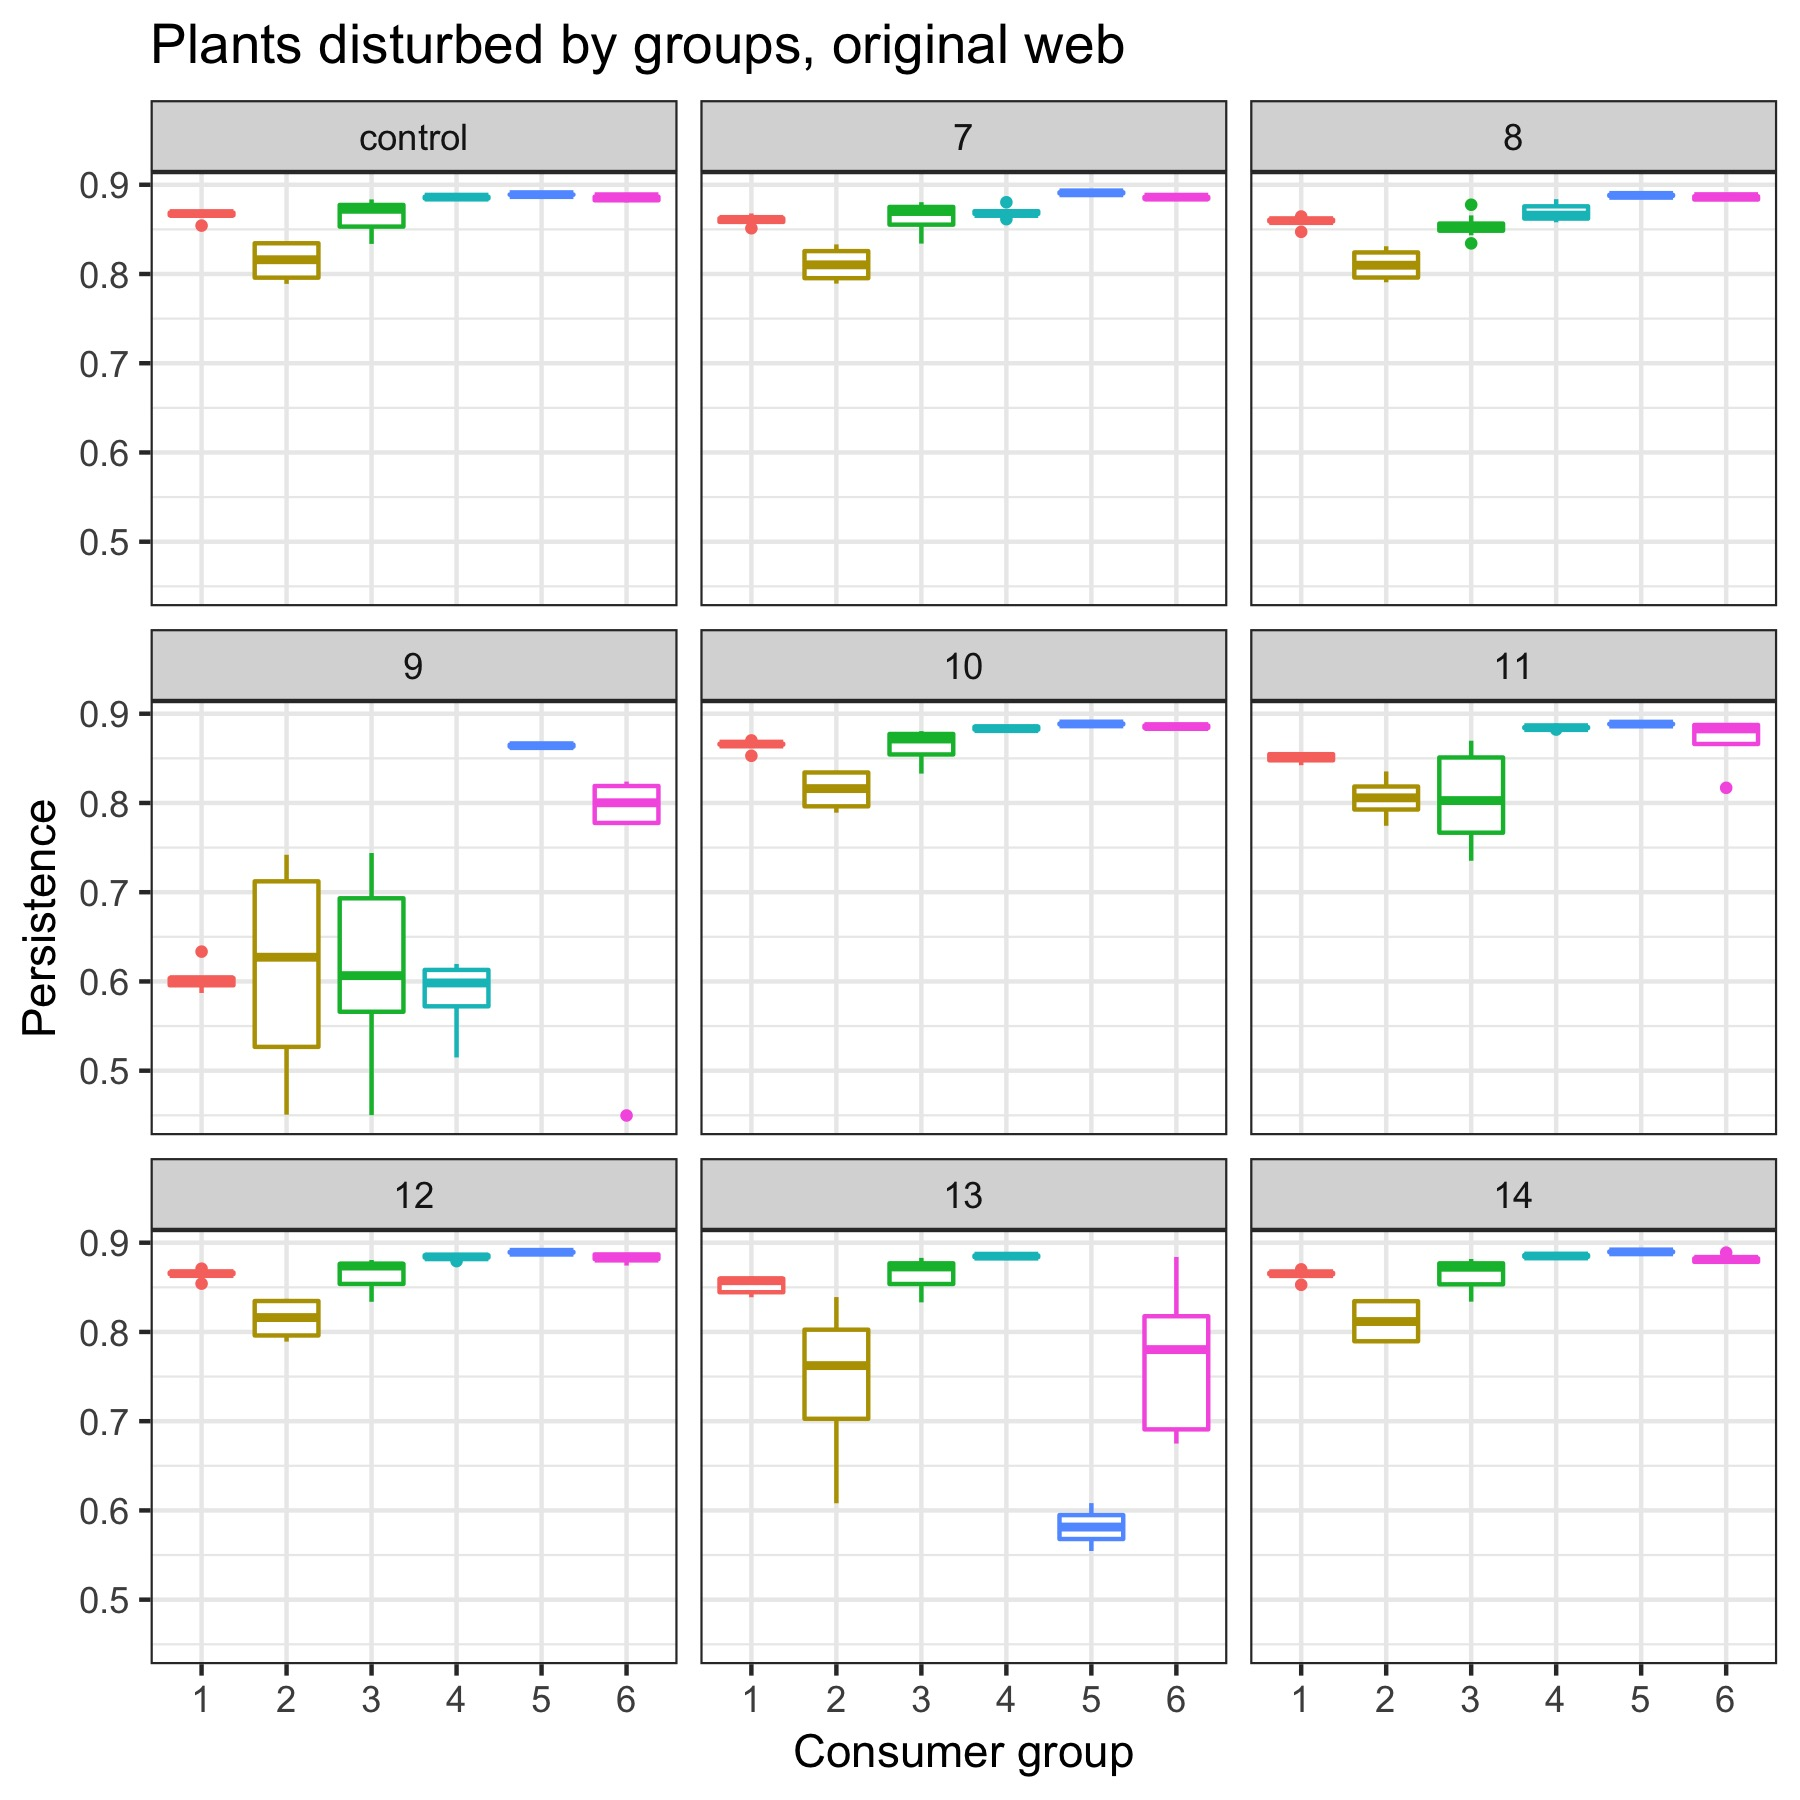
\includegraphics[width=1\textwidth]{../Results/Figures/A3B3/box_orig_groups.jpg}
  \caption{Functional groups of primary producers experience increased baseline probability to persist (sub-panels), and the impact of these disturbances on the persistence (y-axis) of functional groups of consumer species (group 1-6, x-axis) is presented. The first sub-panel shows the persistence without any disturbance on the basal level. The following sub-panels show the effect on groups of consumers when disturbing plant species based on their functional group \citep{Baskervilleetal2011}. The functional response of consumers to the loss of prey species follows a non-linear curve.}.
  \label{fig:groups_nonlinear}
\end{figure}

\begin{figure}[!p]
  \centering
  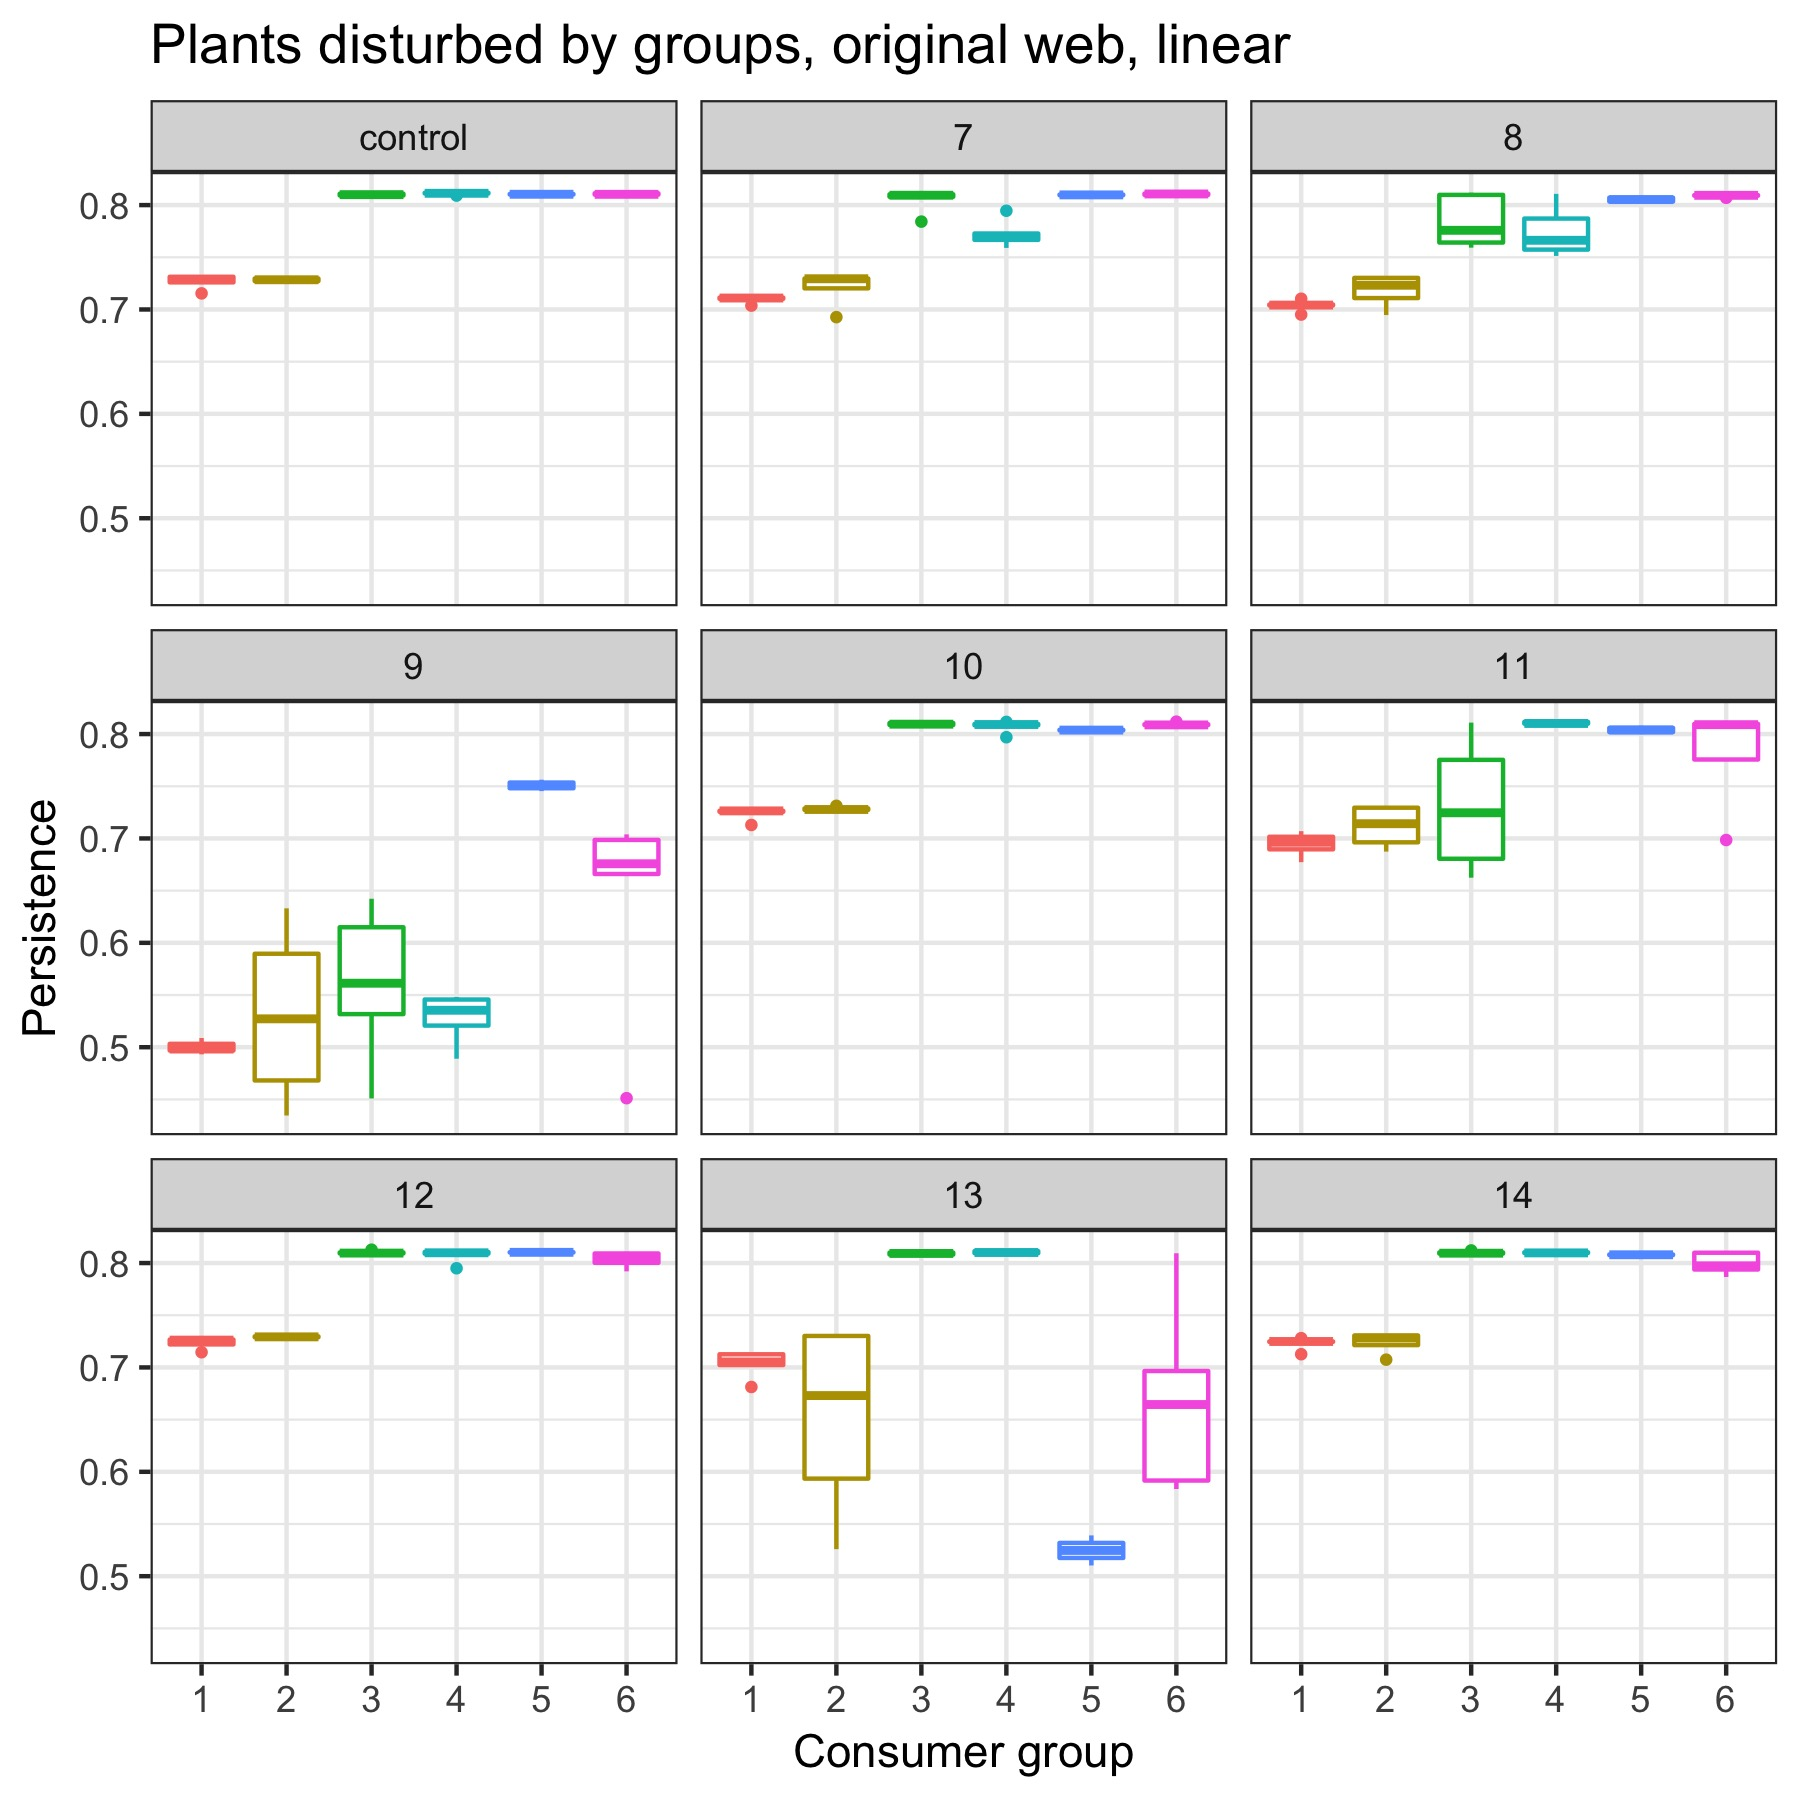
\includegraphics[width=1\textwidth]{../Results/Figures/Linear/box_orig_groups.jpg}
  \caption{Functional groups of primary producers experience increased baseline probability to persist (sub-panels), and the impact of these disturbances on the persistence (y-axis) of functional groups of consumer species (group 1-6, x-axis) is presented. The first sub-panel shows the persistence without any disturbance on the basal level. The following sub-panels show the effect on groups of consumers when disturbing plant species based on their functional group \citep{Baskervilleetal2011}. The functional response of consumers to the loss of prey species follows a linear curve.}.
  \label{fig:groups_linear}
\end{figure}



\begin{figure}[!p]
  \centering
  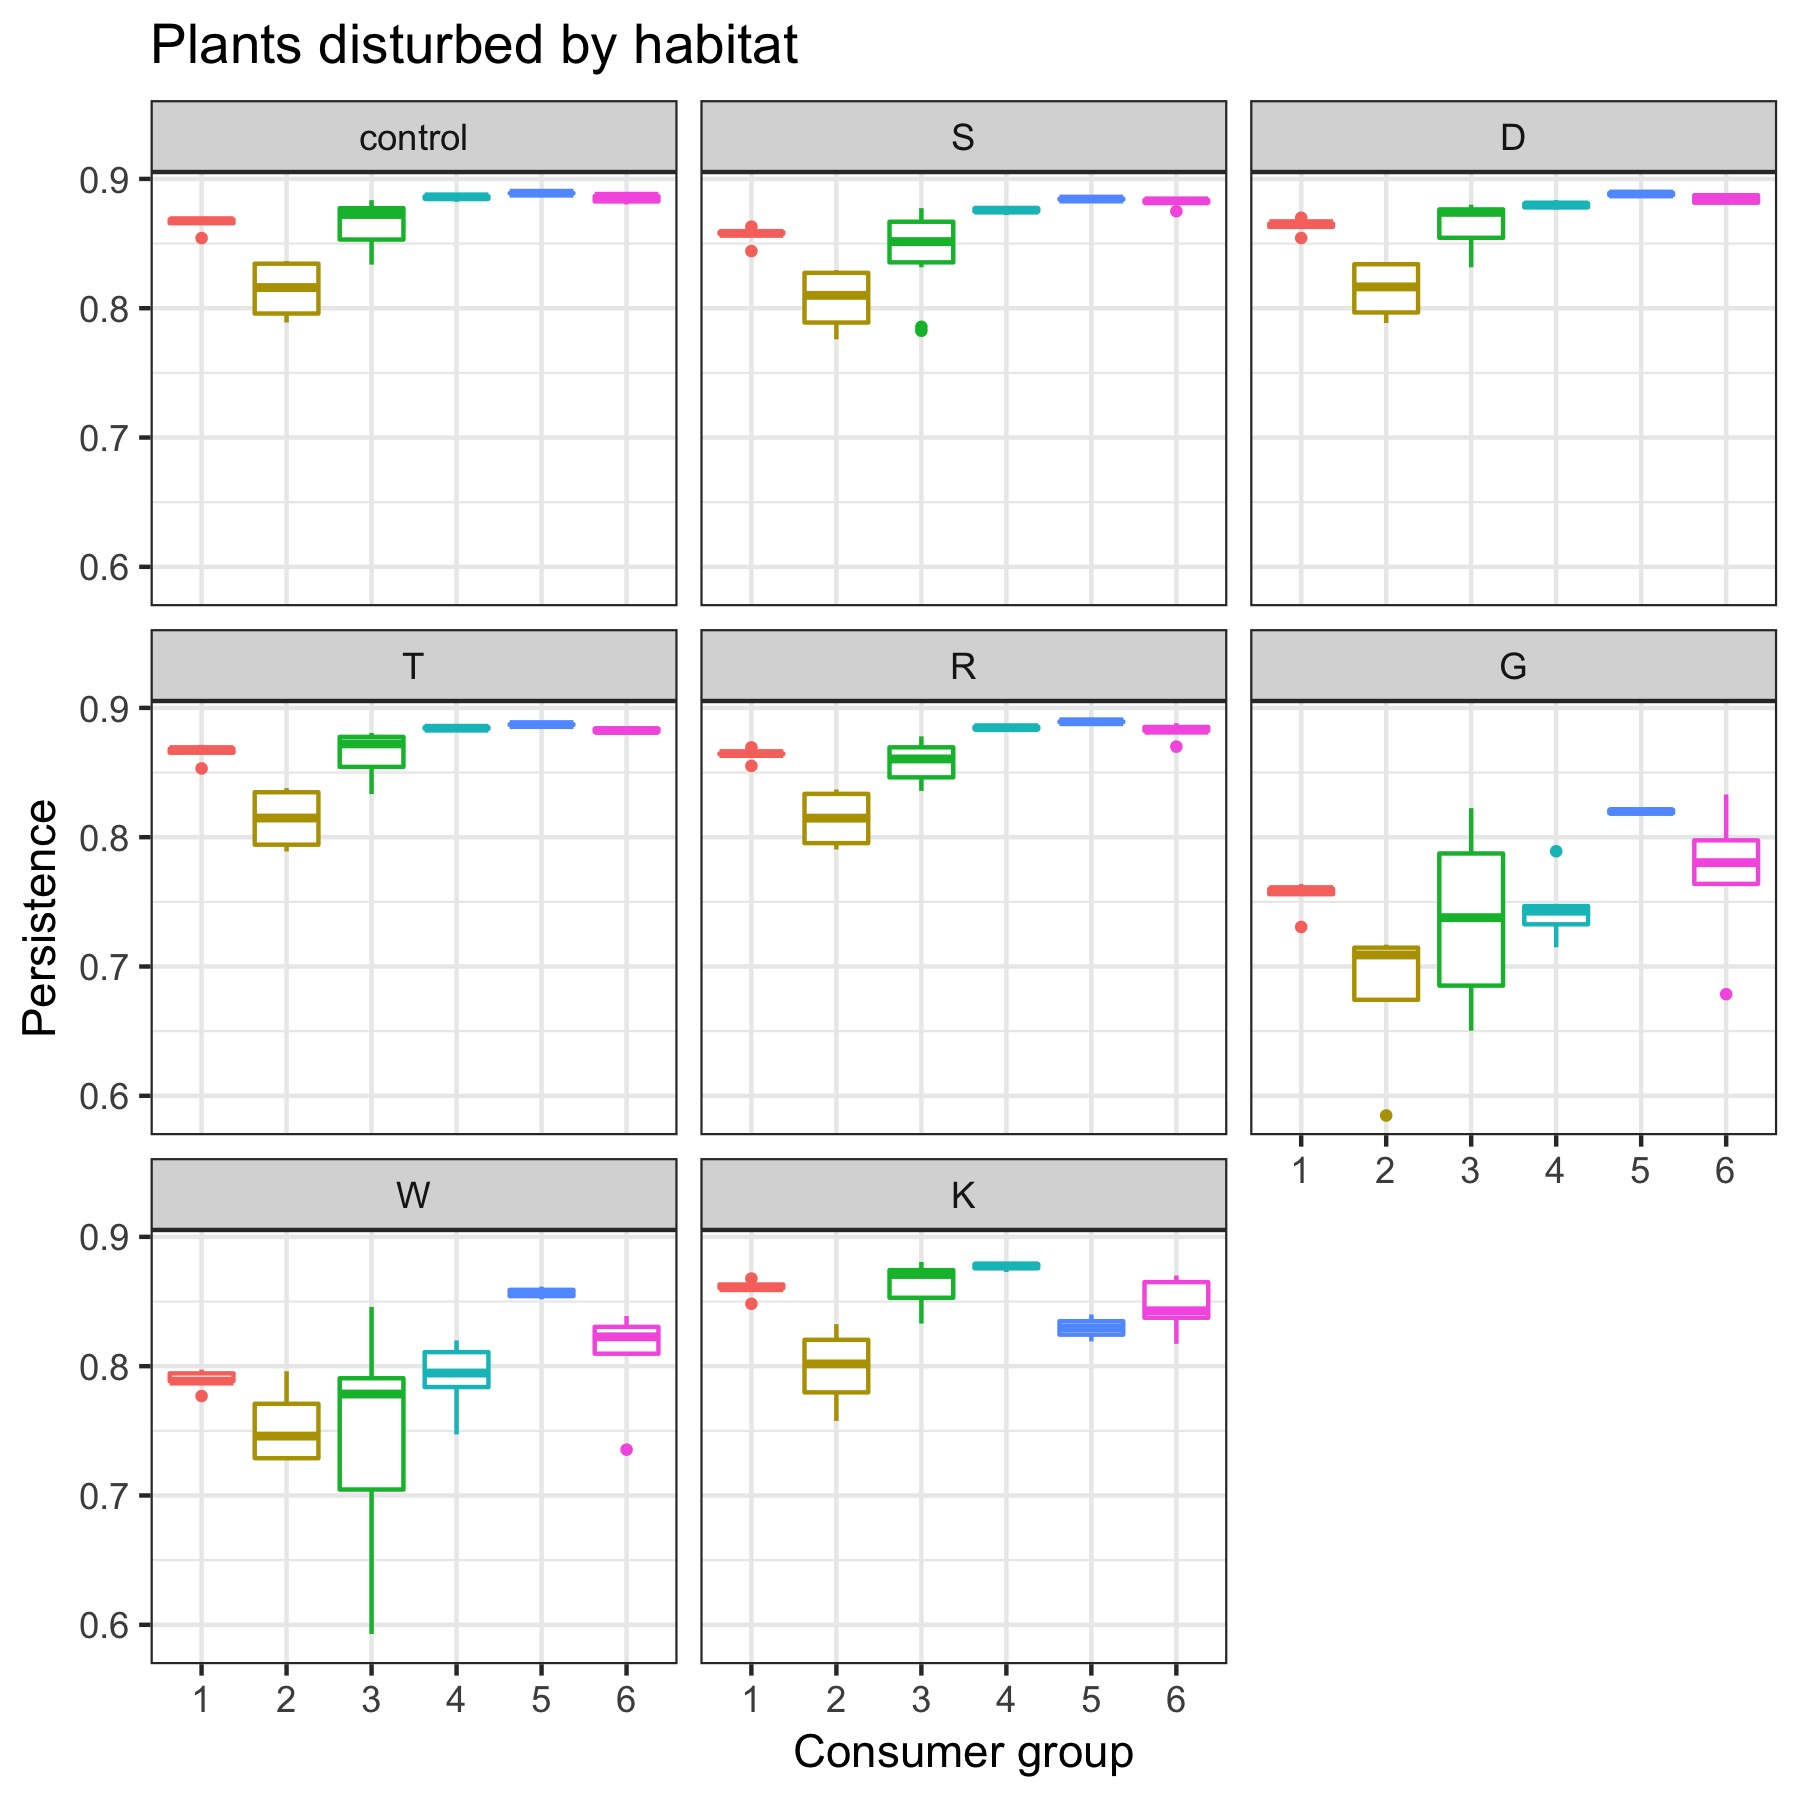
\includegraphics[width=1\textwidth]{../Results/Figures/A3B3/box_orig_habitats.jpg}
  \caption{Impact of disturbances on the basal level based on habitats on groups of consumer species (group 1-6, x-axis). The y-axis shows the probability that the group of consumer will persist. The first sub figure shows the persistence without any disturbance on the basal level. The following sub figures show the effect on groups of consumers when disturbing plant species based on their habitat, indicated by each sub figure's label; S (shrubland), D (disturbed), T (thicket), R (riverland), G (grassland), W (wetland), K (kopje). The functional response of consumers to the loss of prey species follows a non-linear curve.}
  \label{fig:habitats}
\end{figure}

\begin{figure}[!p]
  \centering
  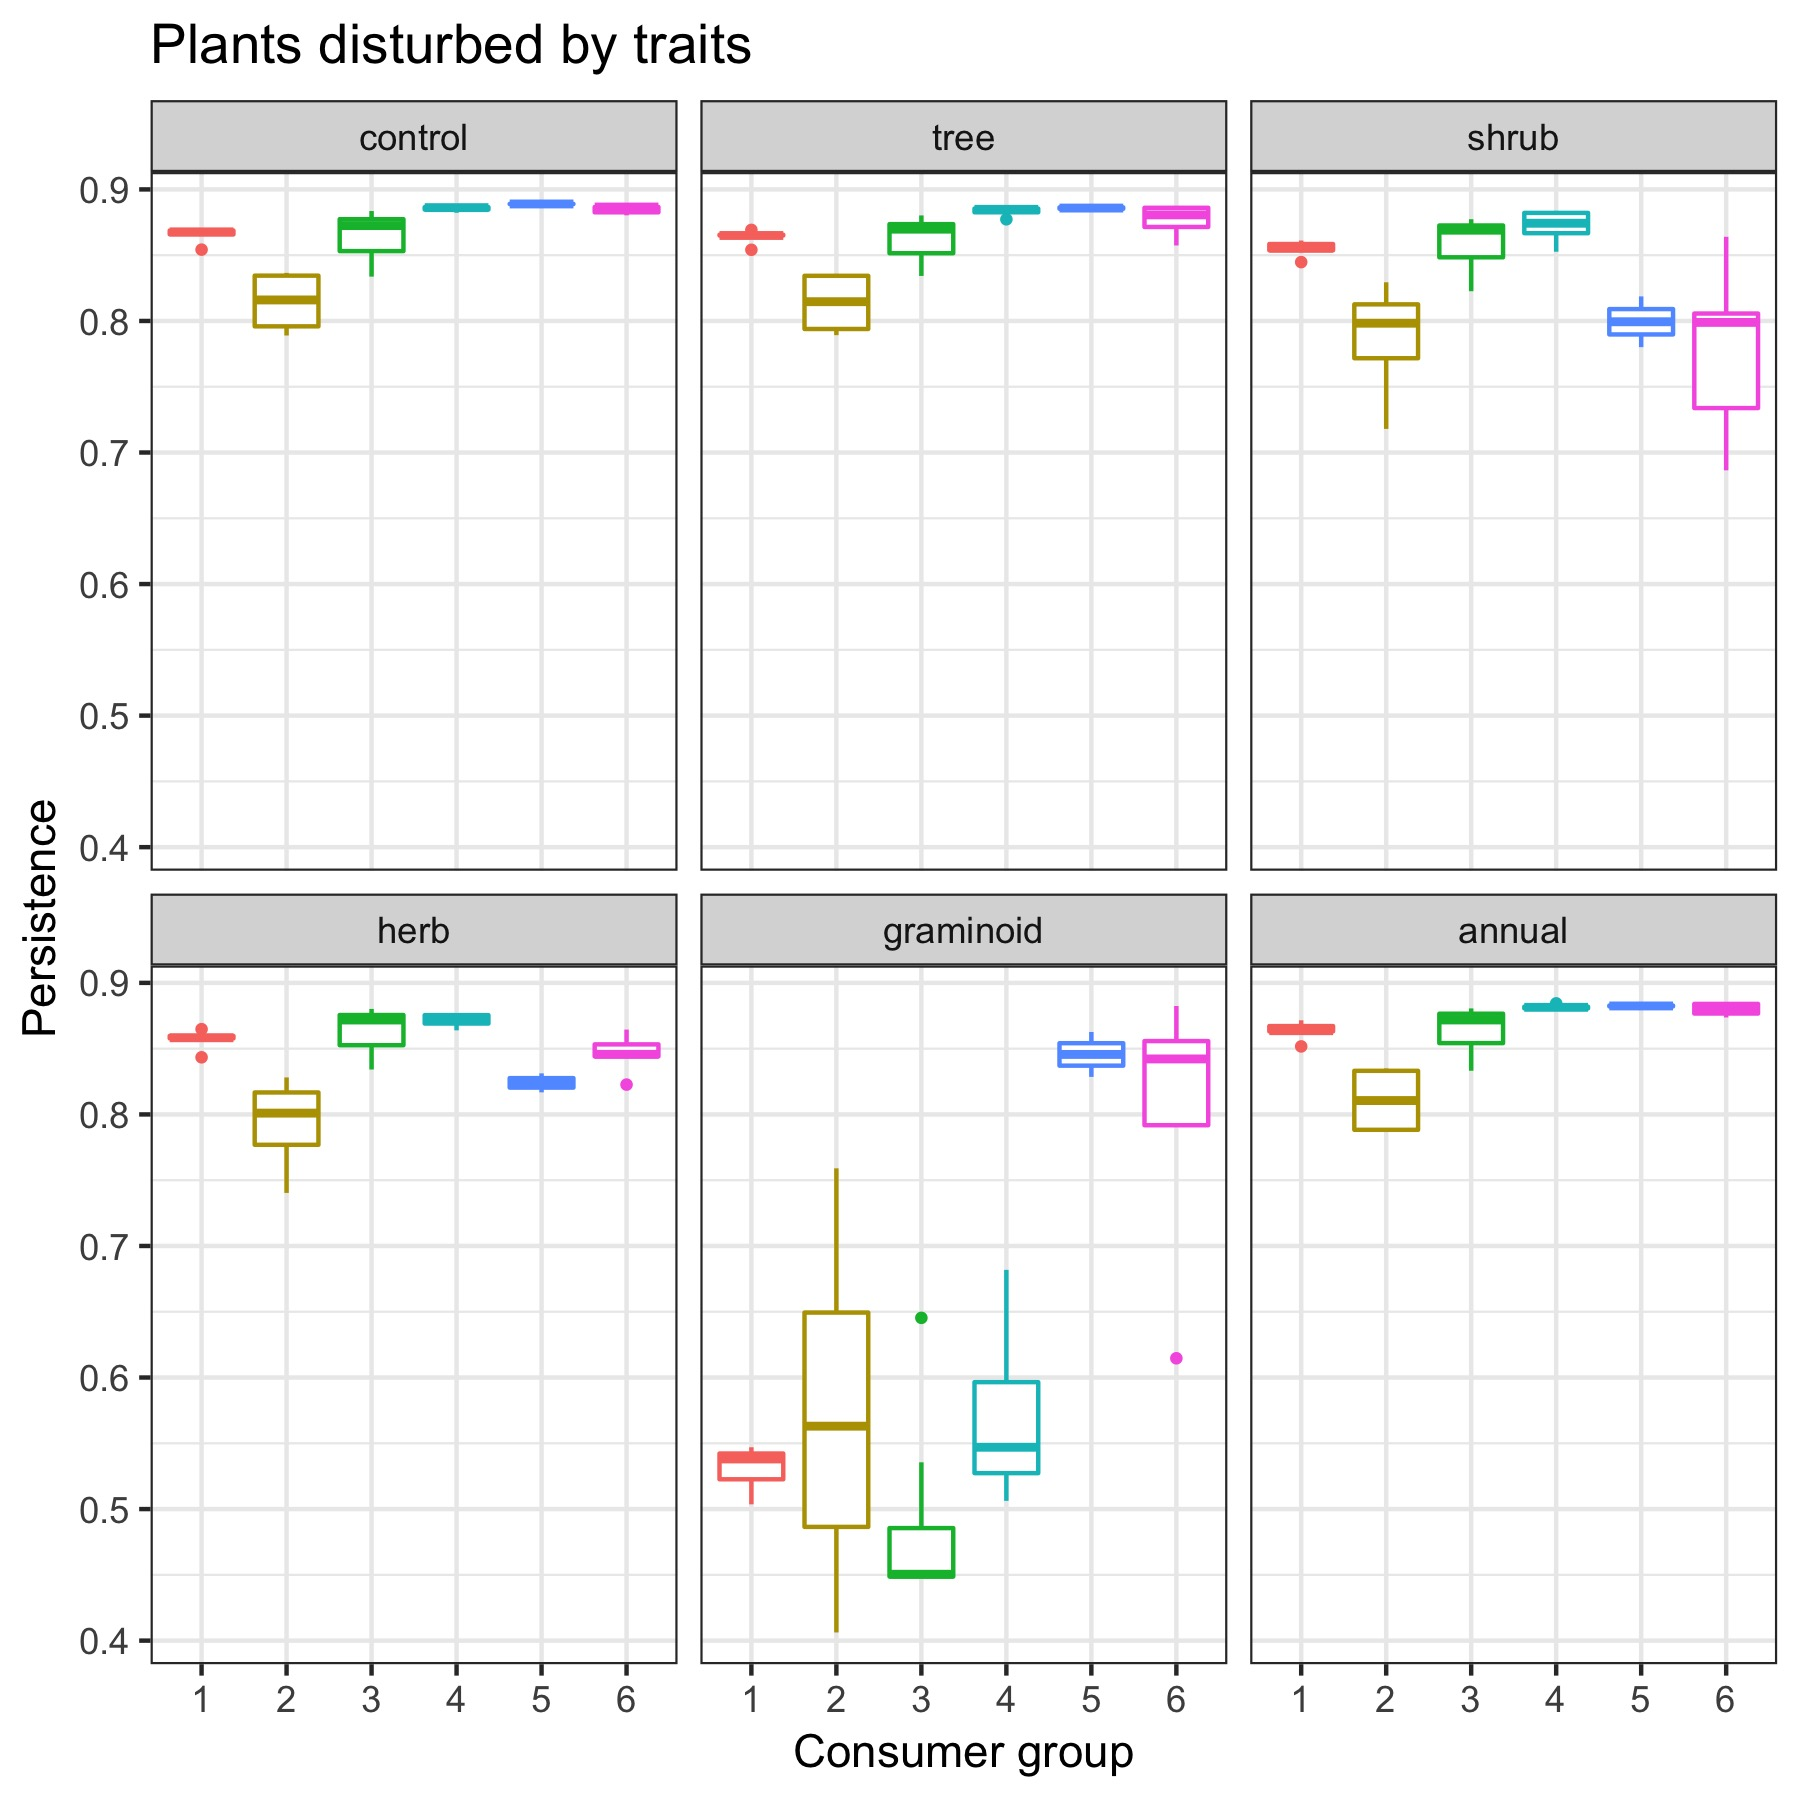
\includegraphics[width=1\textwidth]{../Results/Figures/A3B3/box_orig_traits.jpg}
  \caption{Impact of disturbances on the basal level based on traits on consumer species (group 1-6, x-axis). The y-axis shows the probability that the group of consumer will persist. The first sub figure shows the persistence without any disturbance on the basal level. The following sub figures show the effect on groups of consumers when disturbing plant species based on various traits; tree (large trees), shurb (small trees and shrubs), herbs (herbs and forbs, perennial), graminoid (grasses), annual (annual flowering plants). The functional response of consumers to the loss of prey species follows a non-linear curve.}
  \label{fig:traits}
\end{figure}
 
\begin{figure}[!p]
  \centering
  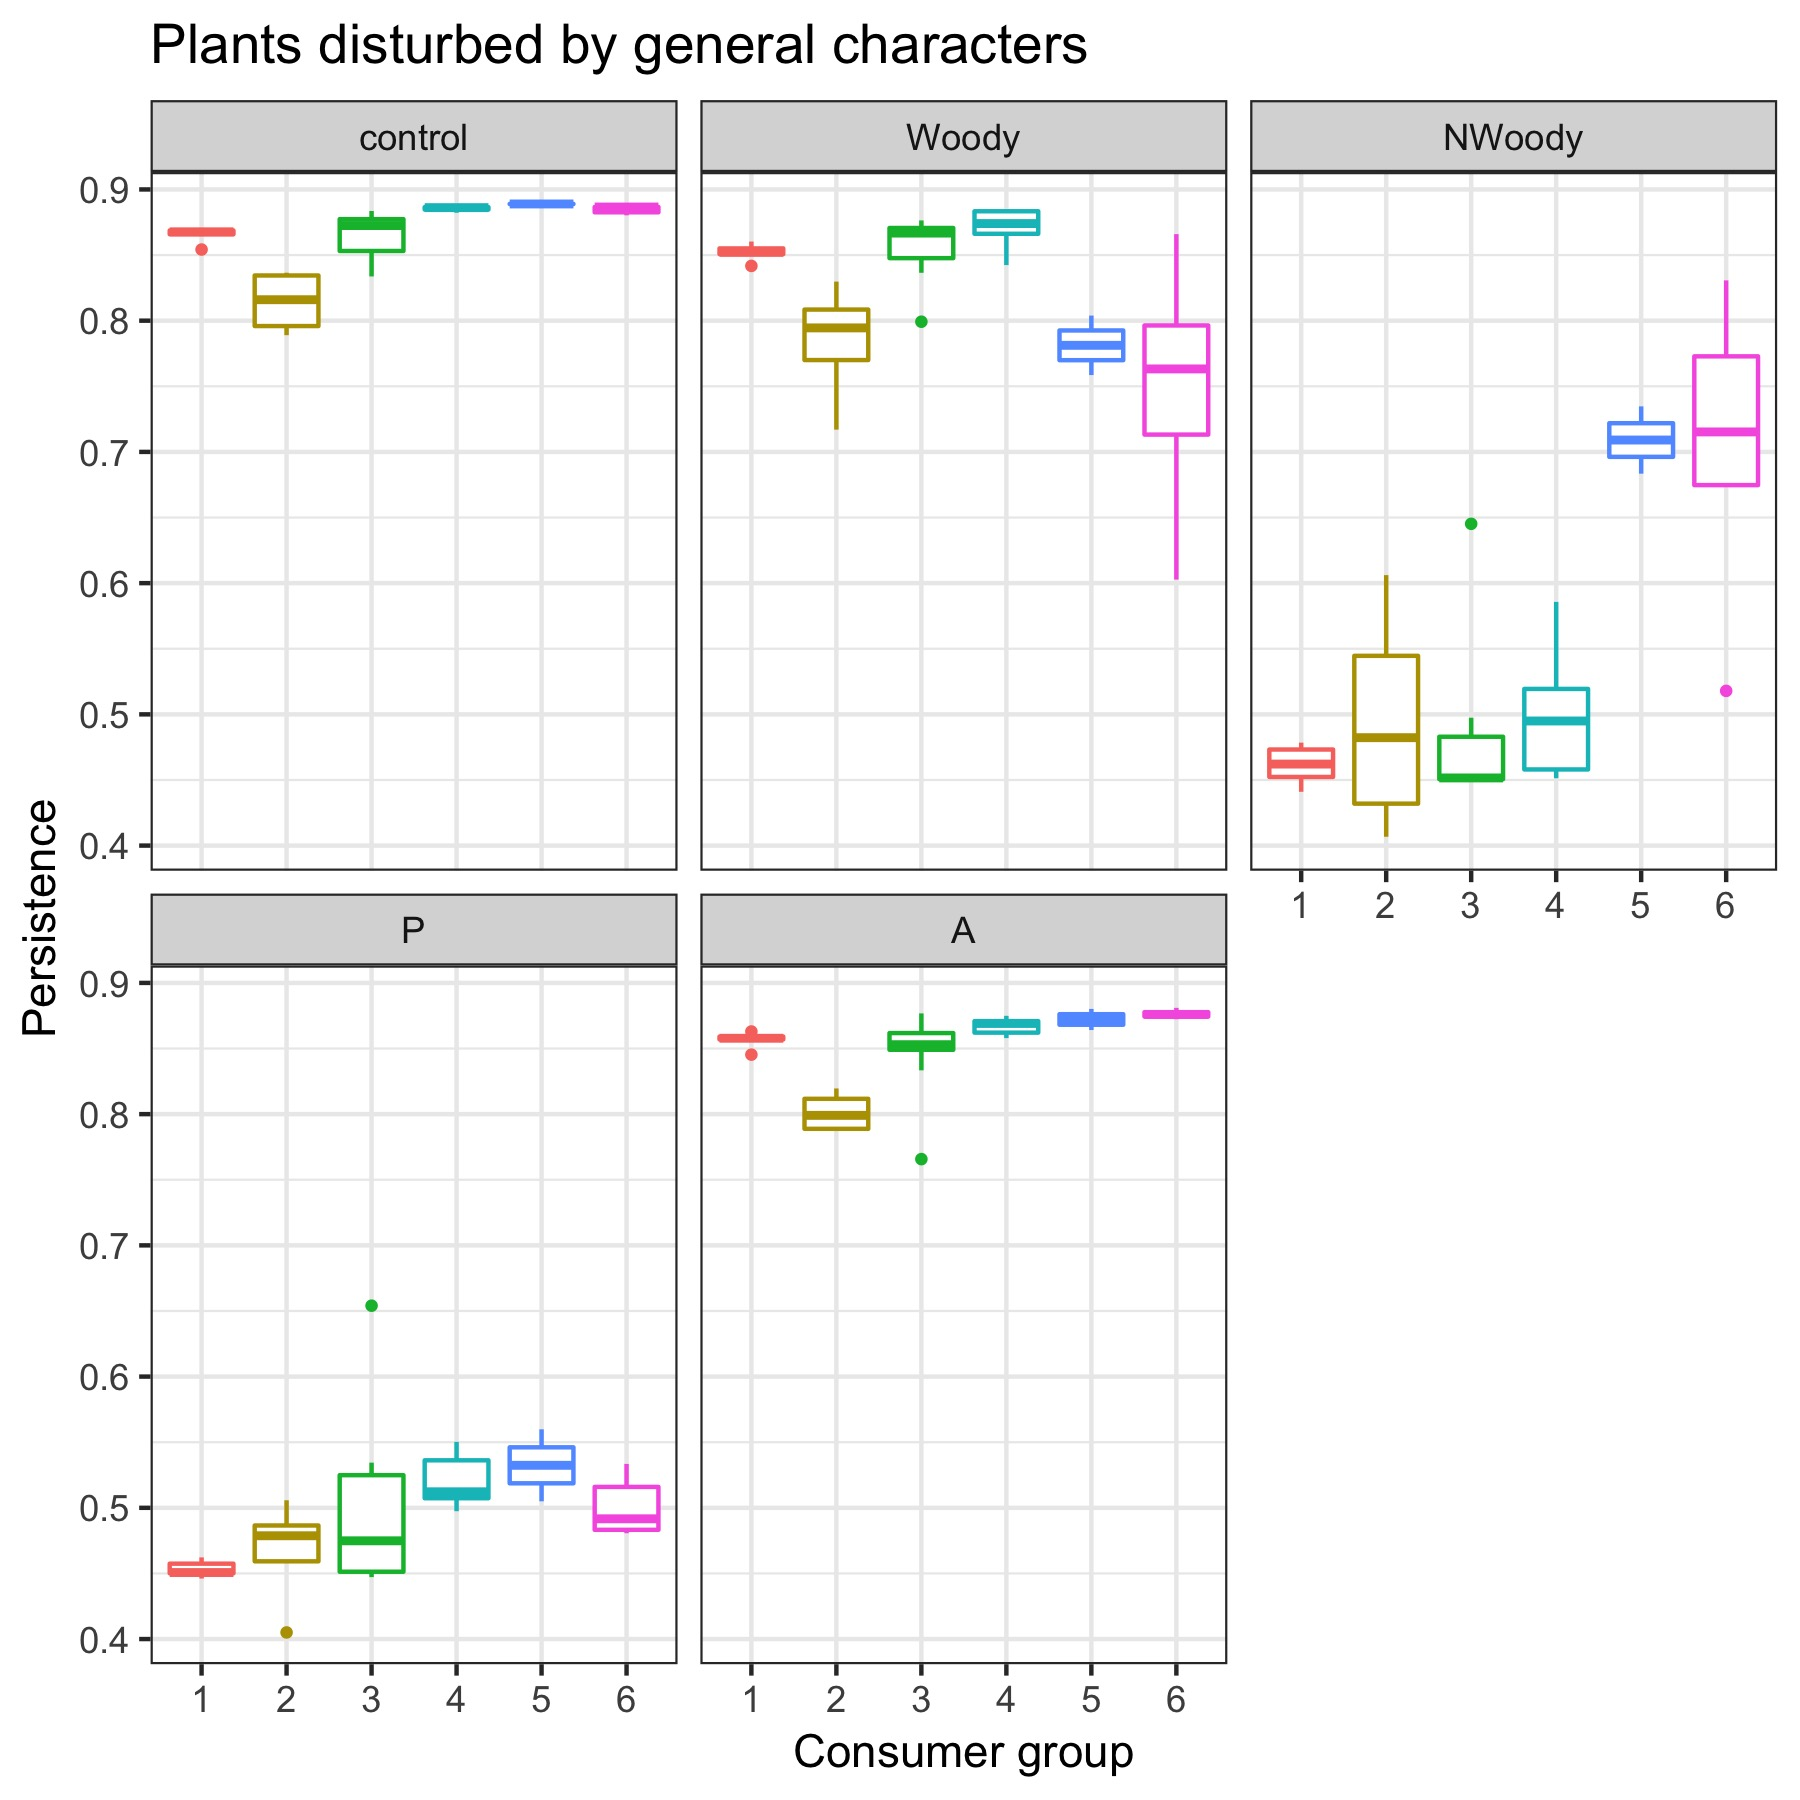
\includegraphics[width=1\textwidth]{../Results/Figures/A3B3/box_orig_gen_charac.jpg}
  \caption{Impact of disturbances on the basal level based on traits on consumer species (group 1-6, x-axis). The y-axis shows the probability that the group of consumer will persist. The first sub figure shows the persistence without any disturbance on the basal level. The following sub figures show the effect on groups of consumers when disturbing plant species based on various traits; woody (woody plants), Nwoody (non-woody plants), P (perennials), A (annuals). The functional response of consumers to the loss of prey species follows a non-linear curve.}
  \label{fig:gen_charac}
\end{figure}

\begin{figure}[!p]
  \centering
  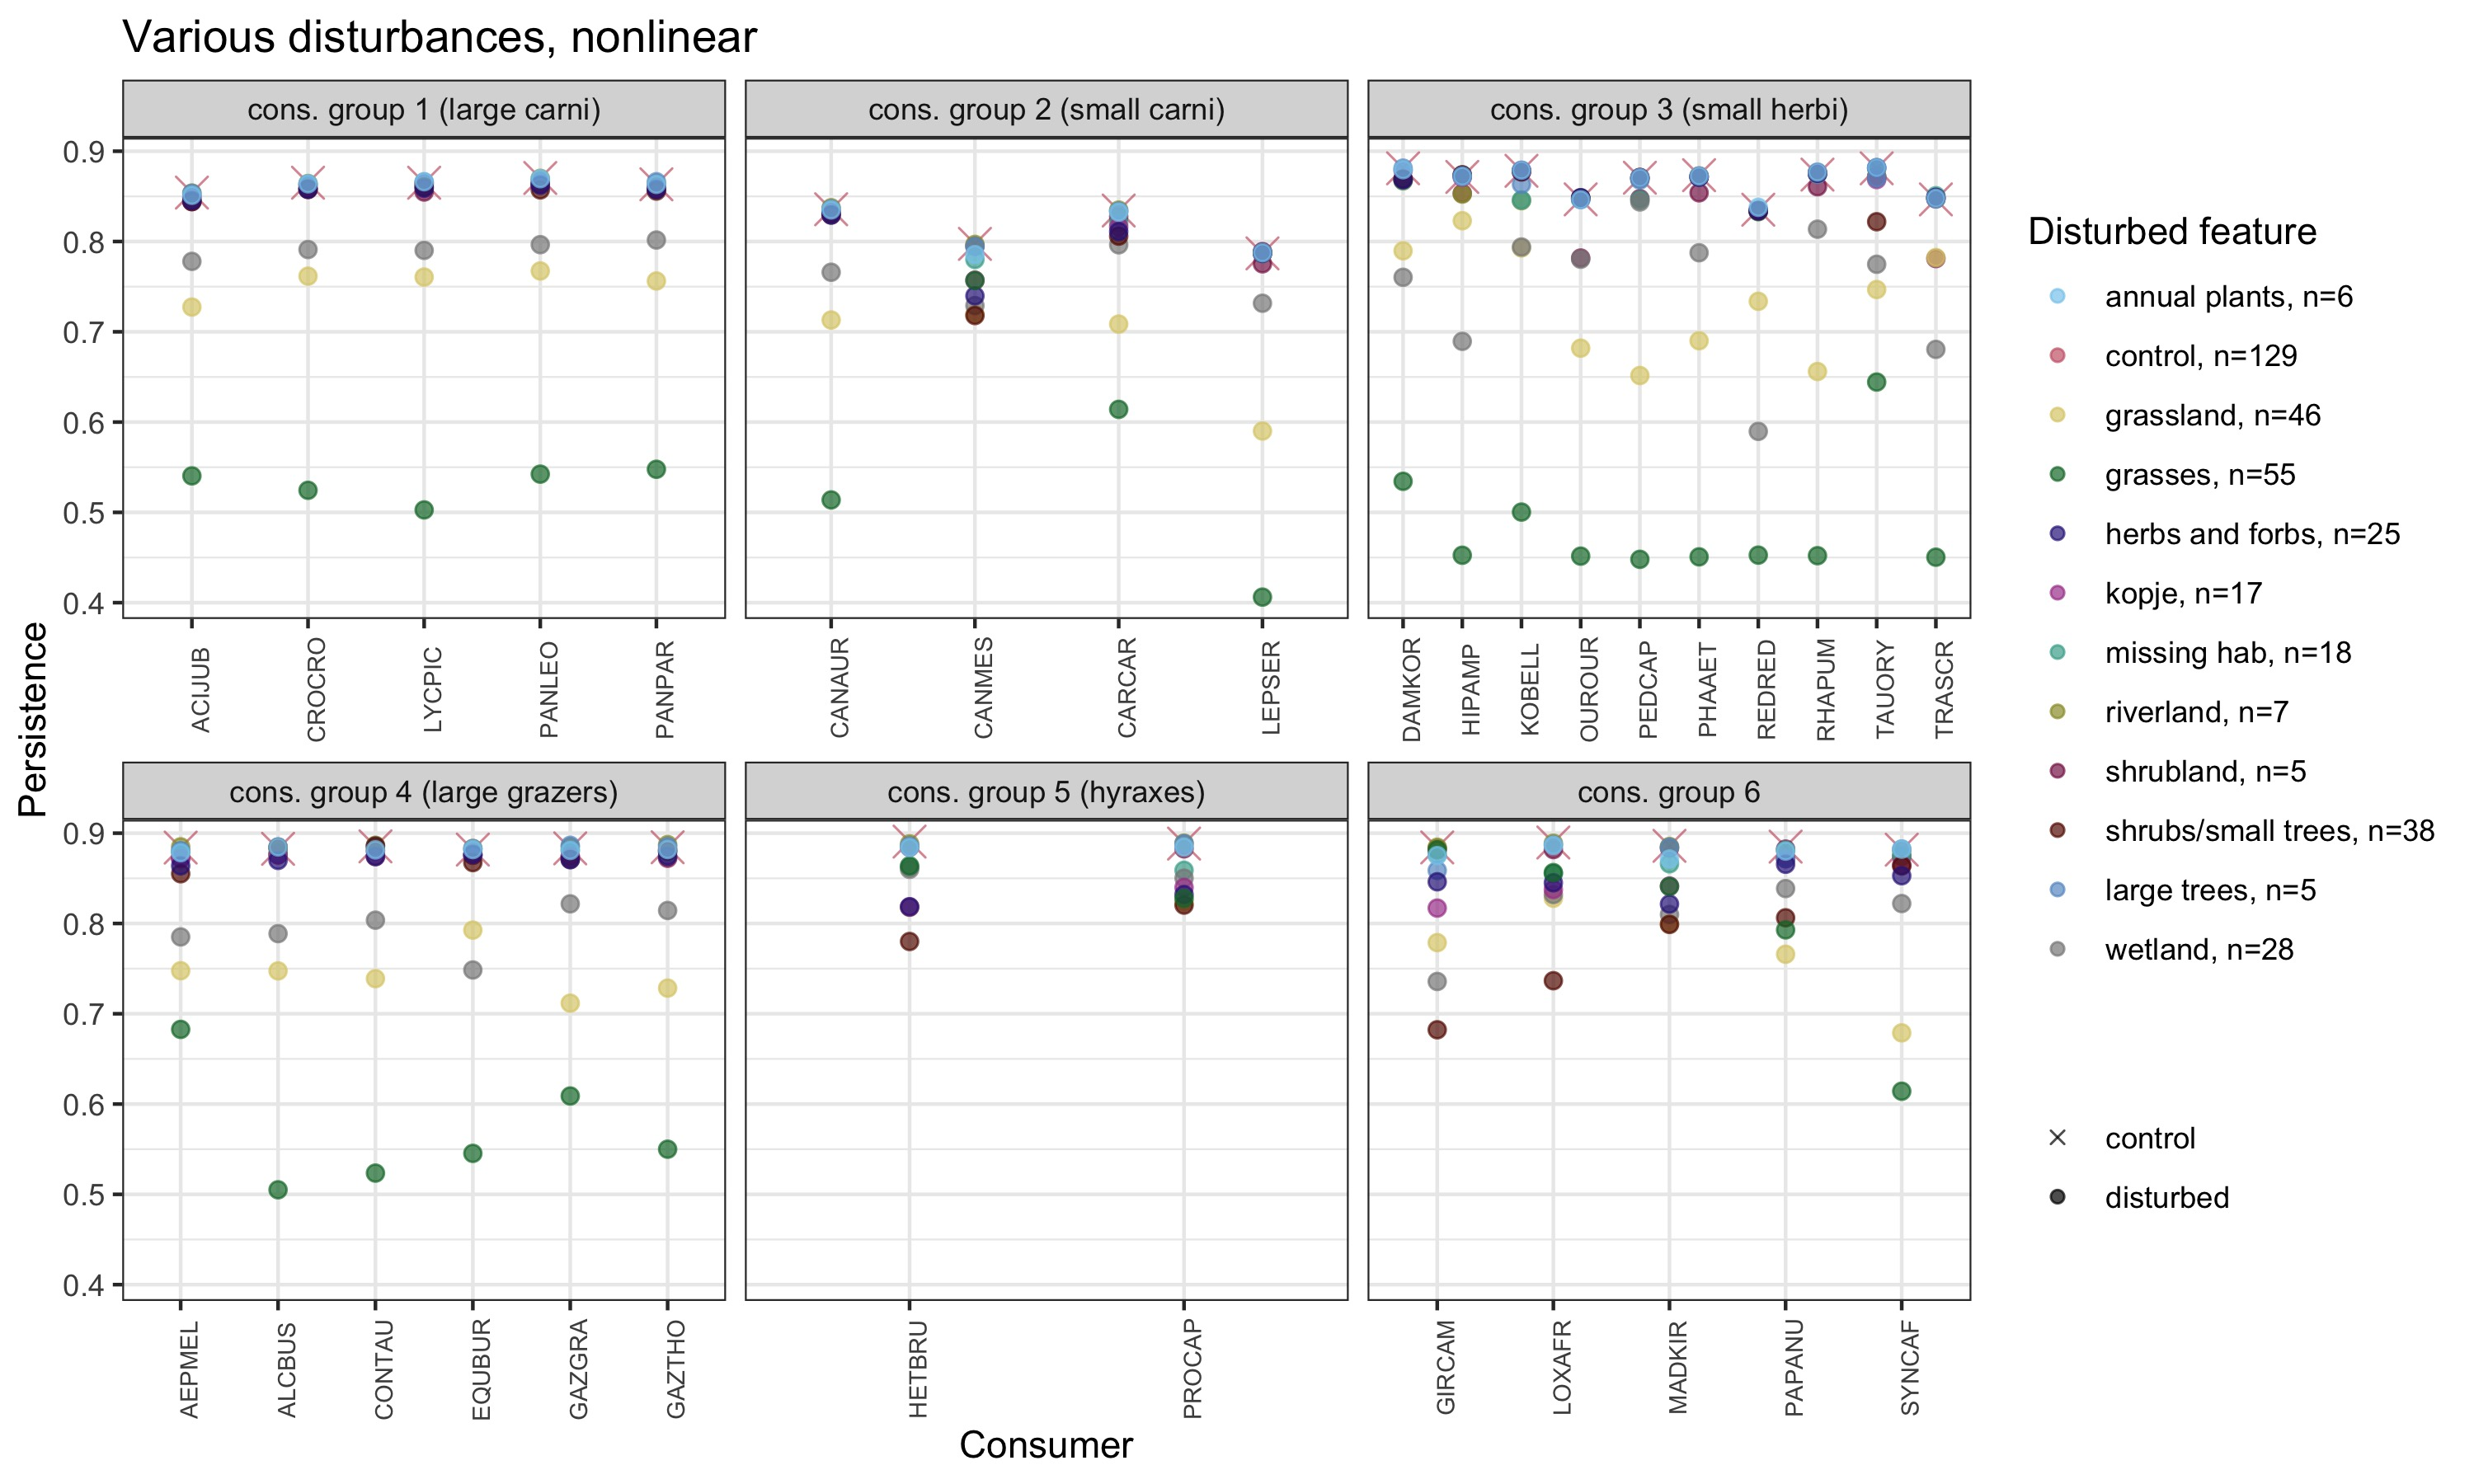
\includegraphics[width=1\textwidth]{../Results/Figures/A3B3/disturb.jpg}
  \caption{Impact of disturbances on the basal level based on traits and habitats on consumer species (group 1-6, panels). The y-axis shows the probability of persistence for each consumer species. The control scenario, without any additional disturbances, is indicated in each sub-figure by the shape "x", disturbance scenarios by circles. The colors represent various disturbance scenarios, described in the legend, also showing the number (n) of plant species being disturbed in each particular scenario. The functional response of consumers to the loss of prey species follows a non-linear curve.}
  \label{fig:all_disturbances}
\end{figure}

\begin{figure}[!p]
  \centering
  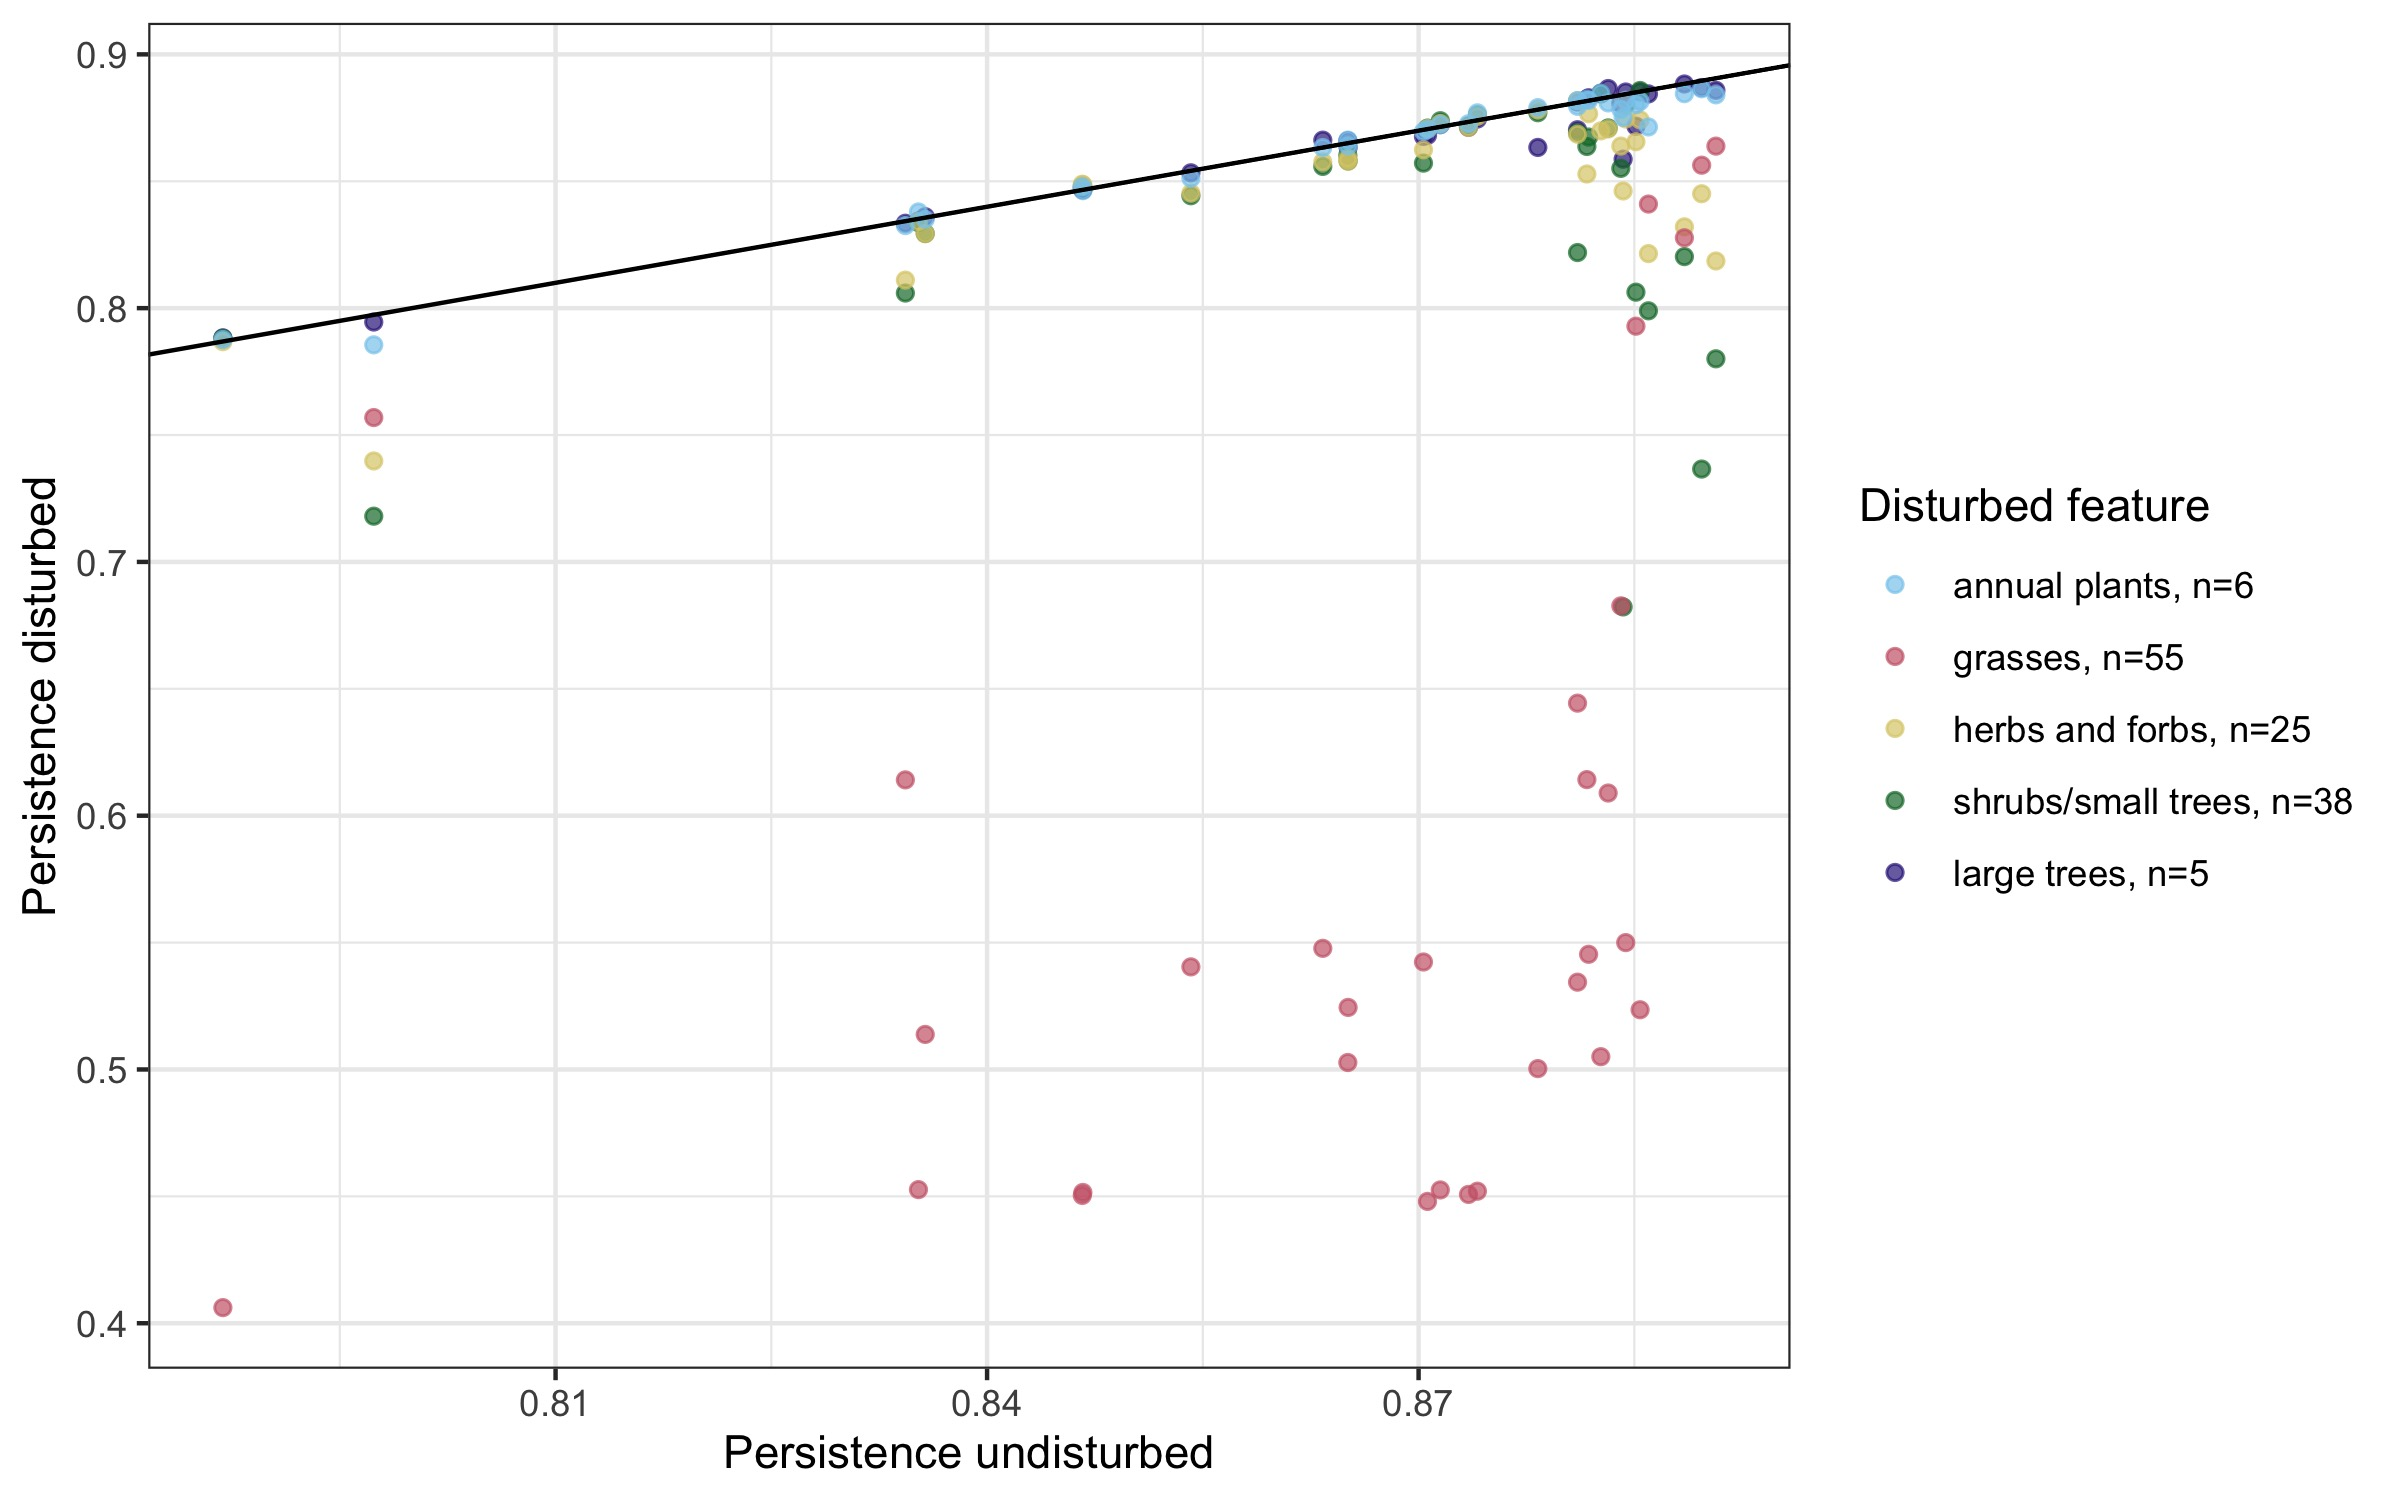
\includegraphics[width=1\textwidth]{../Results/Figures/A3B3/comp_traits.jpg}
  \caption{Comparison of persistences in the undisturbed, control scenario (x-axis), and the various disturbance scenarios focusing on plant species traits (y-axis). Values on the line indicate that similar persistences are reached independent of disturbances on the plant level. Values below the line show that persistences are lower in the disturbed scenario than in the control scenario. The colors show the various traits disturbed presented in the legend, as well as the number of plant species (n) disturbed in each scenario. The functional response of consumers to the loss of prey species follows a non-linear curve.}
  \label{fig:comp_dist_traits}
\end{figure}

\begin{figure}[!p]
  \centering
  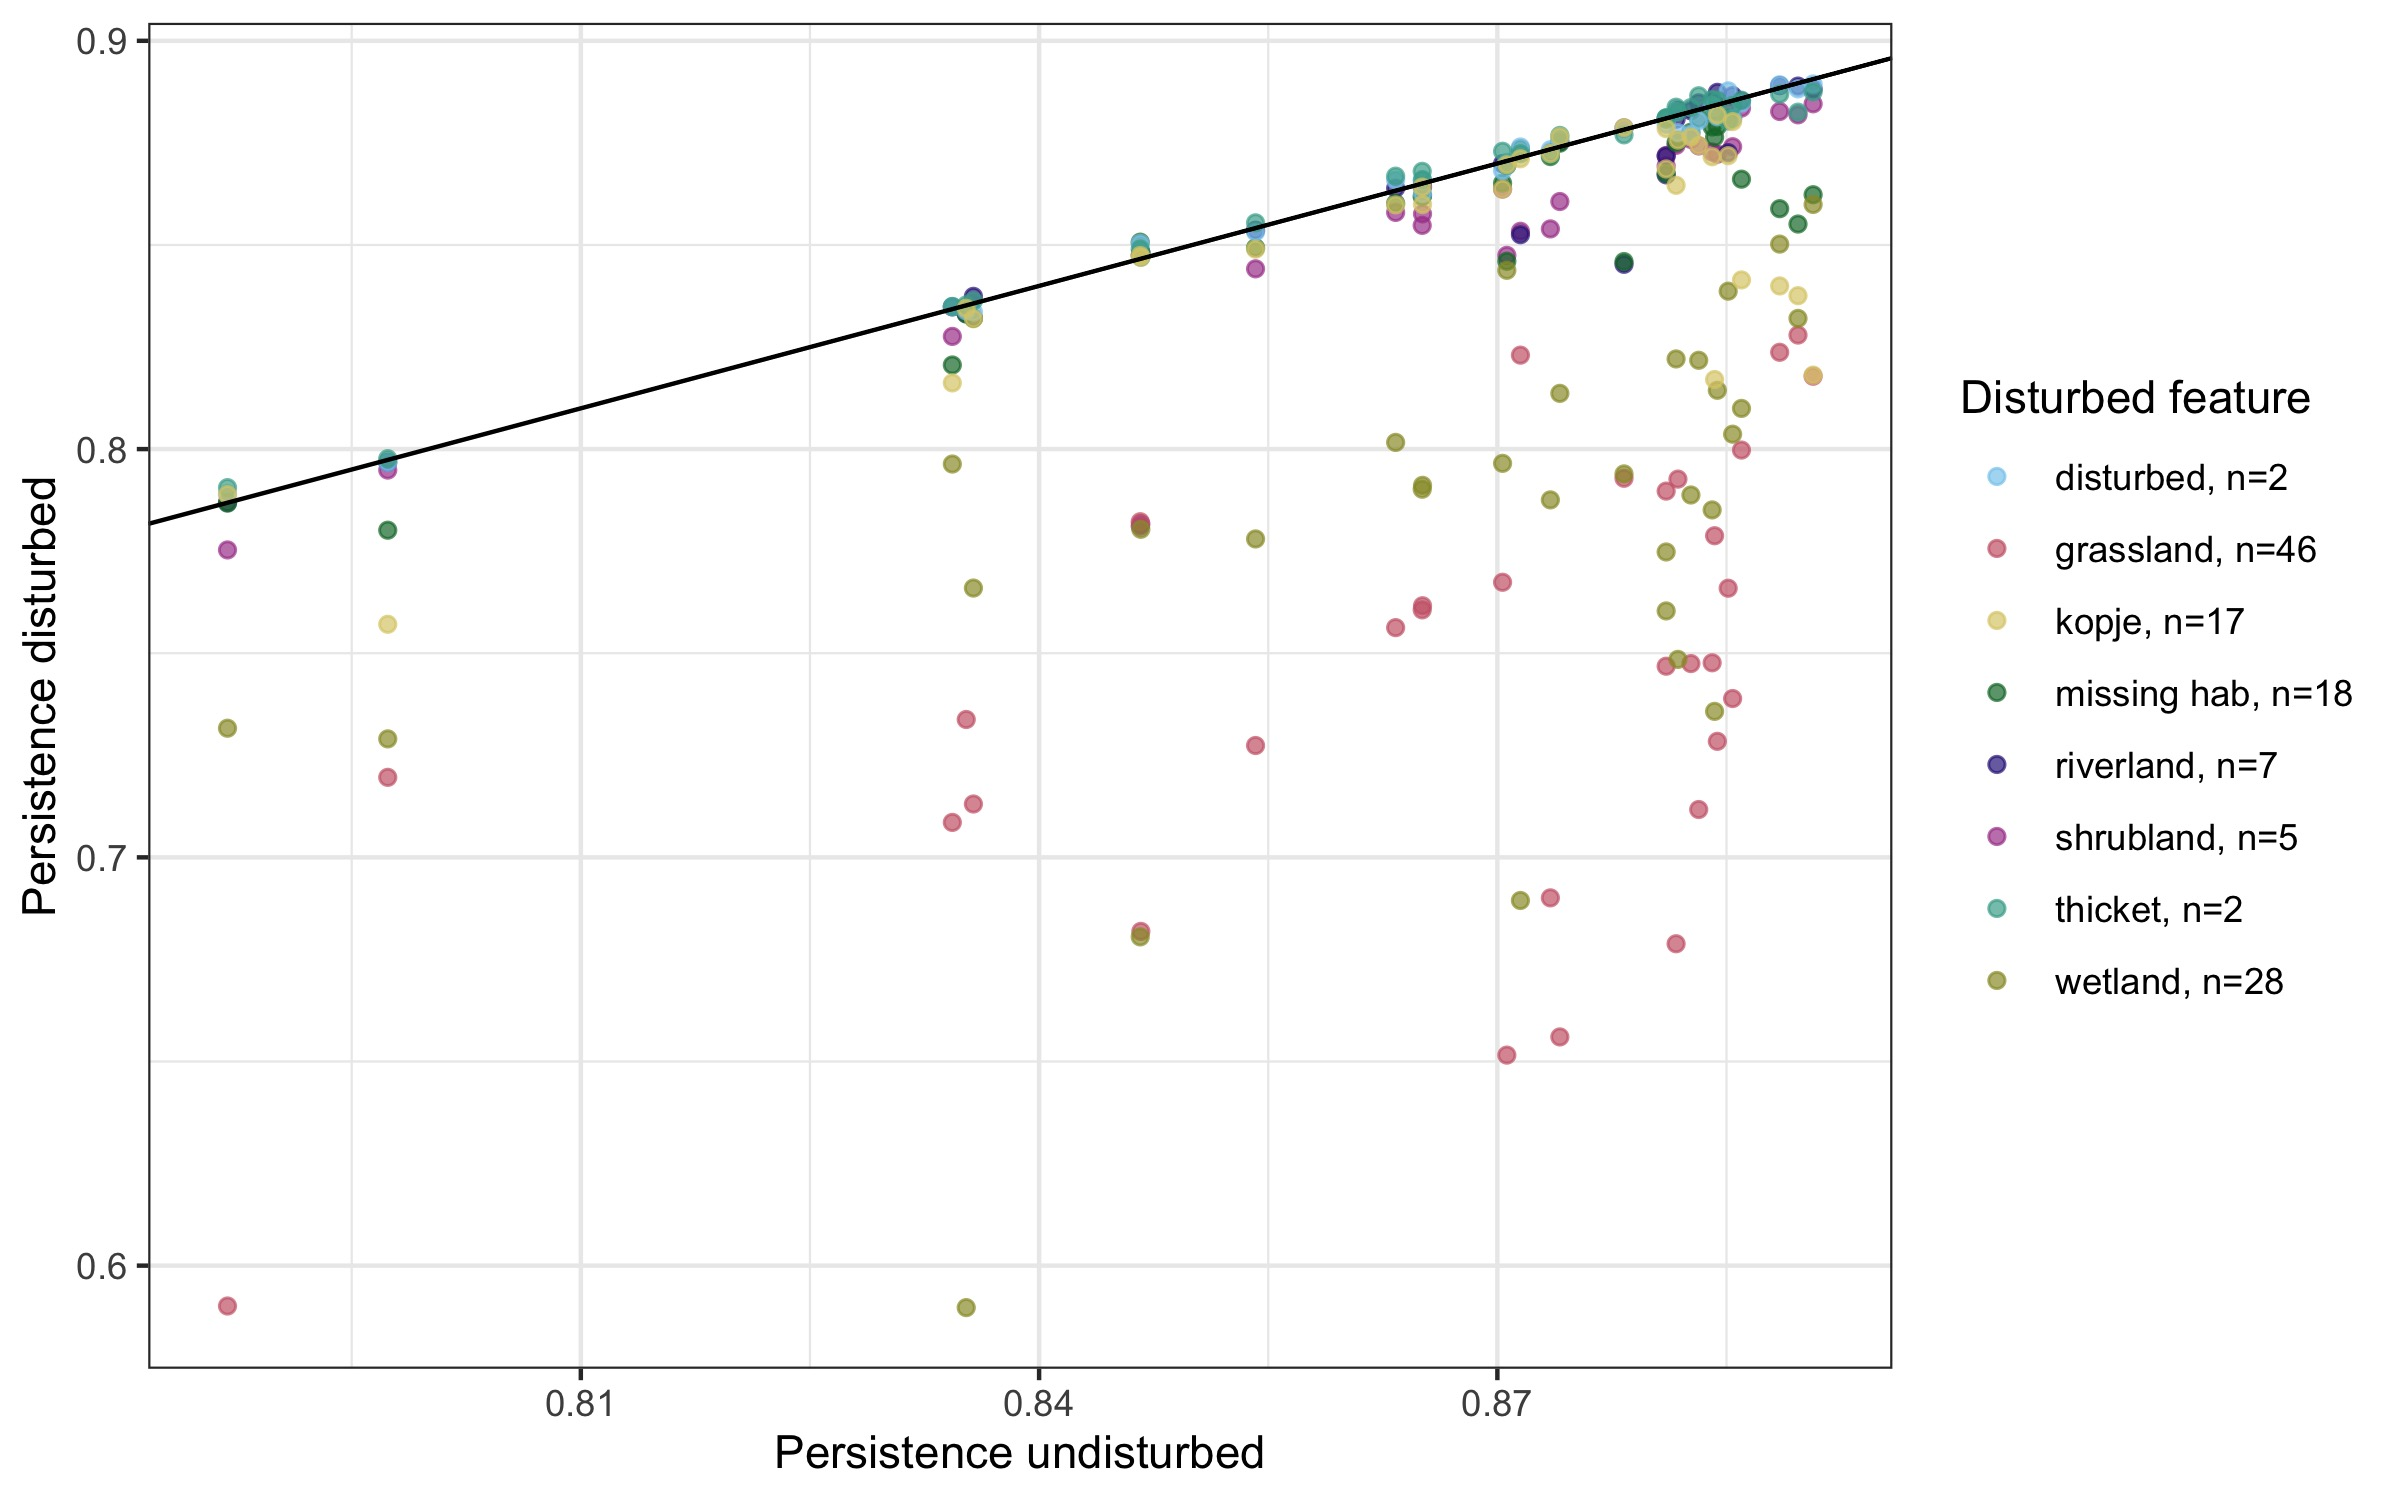
\includegraphics[width=1\textwidth]{../Results/Figures/A3B3/comp_habs.jpg}
  \caption{Comparison of persistences in the undisturbed, control scenario (x-axis), and various disturbance scenarios of habitats (y-axis). Values on the line indicate that similar persistences are reached independent of disturbances on the plant level. Values below the line indicate lower persistences in the disturbed scenario than in the control scenario. The colors show the various traits disturbed presented in the legend, as well as the number of plant species (n) disturbed in each scenario. The functional response of consumers to the loss of prey species follows a non-linear curve.}
  \label{fig:comp_dist_habs}
\end{figure}


\begin{figure}[!p]
  \centering
  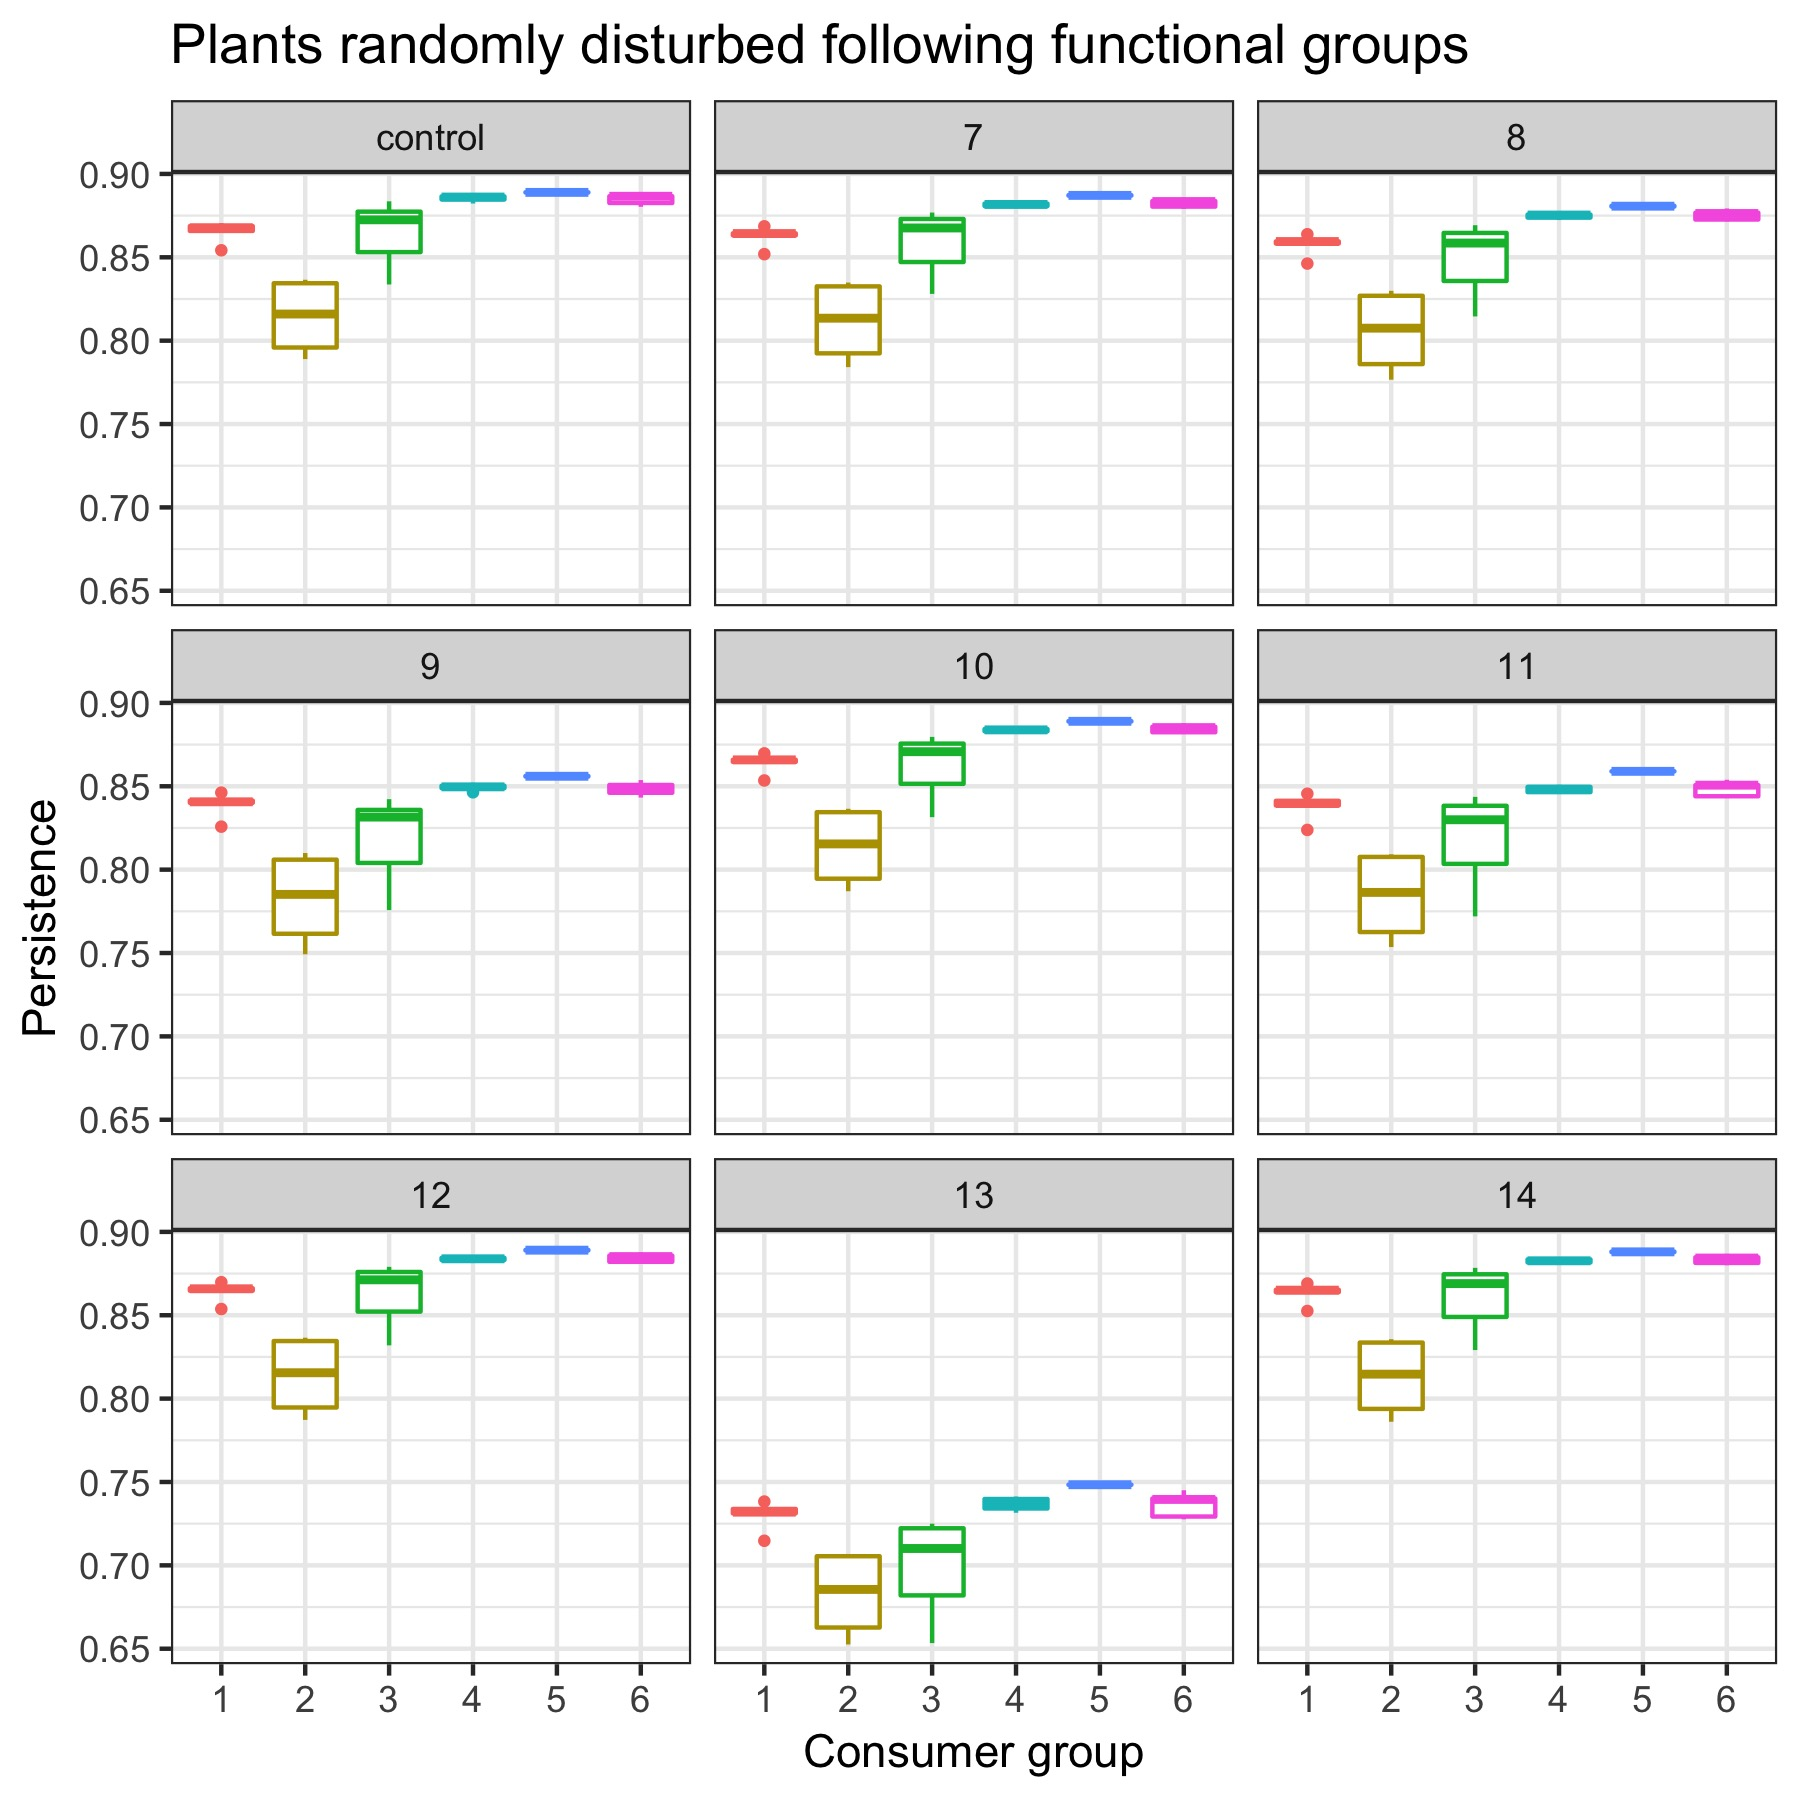
\includegraphics[width=1\textwidth]{../Results/Figures/A3B3/random/box_orig_random_groups.jpg}
  \caption{Disturbance of groups of randomly chosen plant species, corresponding to the size of the functional plant groups identified by Baskerville et al. \citep{Baskervilleetal2011}. The first sub-panel shows the persistence without any disturbance on the basal level. The following sub-panels show disturbance of random plant groups, numbered by the original functional group, containing the same number of species. The impact of these disturbances on the persistence (y-axis) of functional groups of consumer species (group 1-6, x-axis) is presented. The functional response of consumers to the loss of prey species follows a non-linear curve.}
  \label{fig:random_nonlinear}
\end{figure}

\begin{figure}[!p]
  \centering
  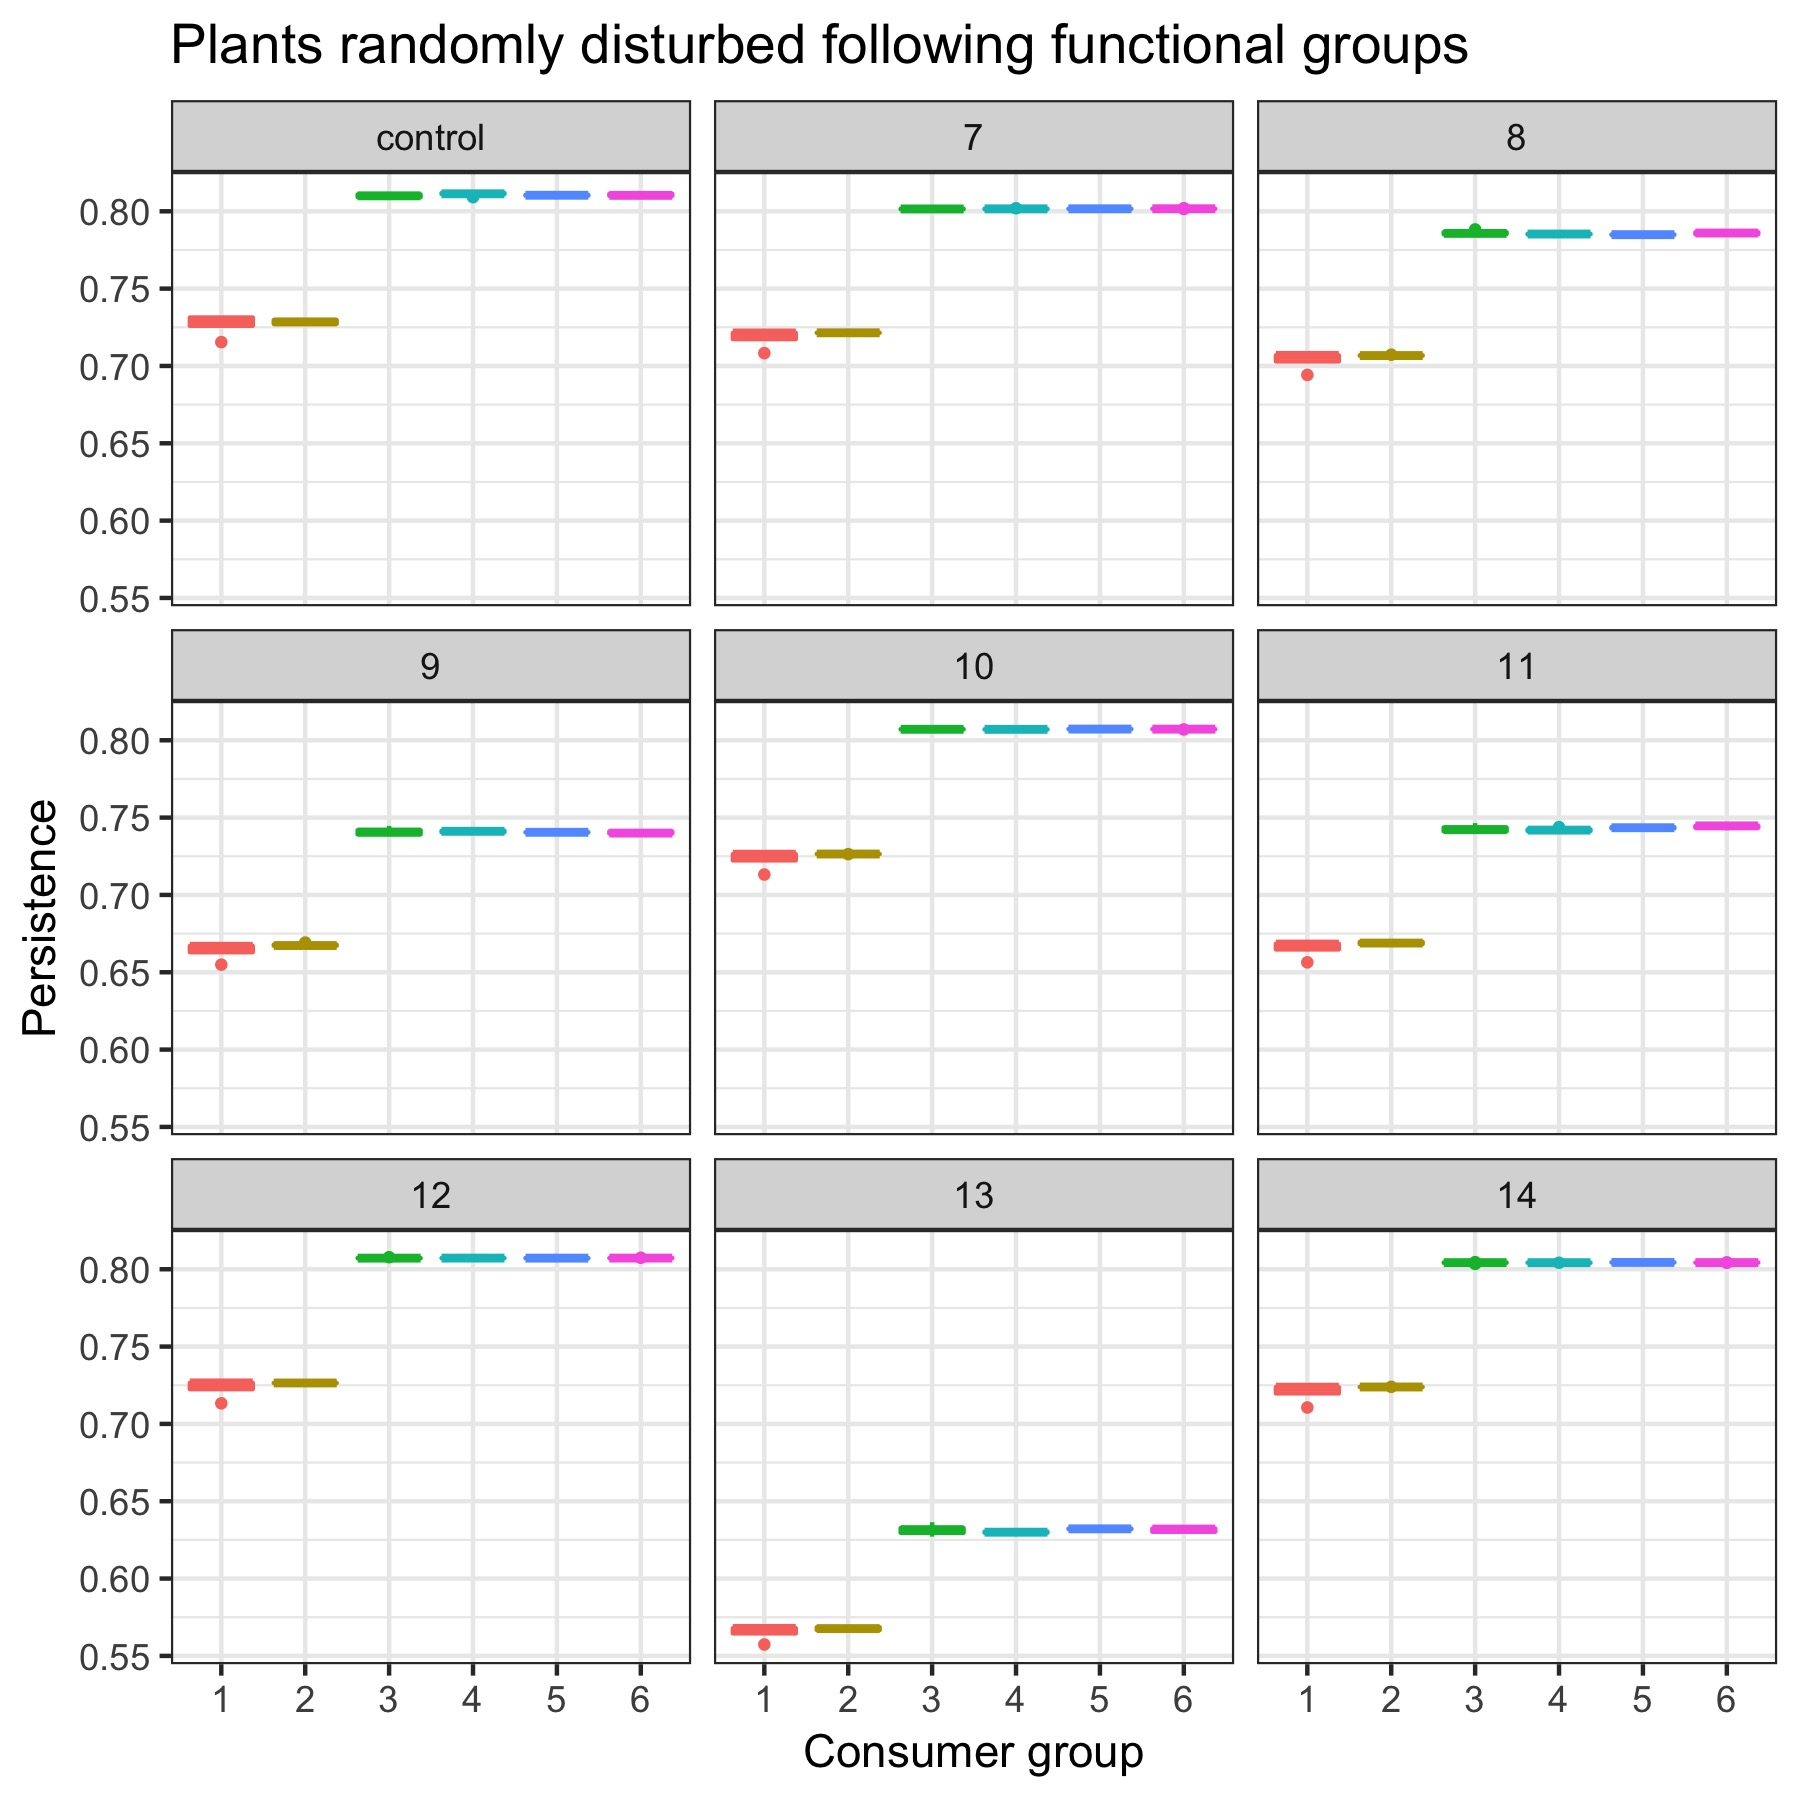
\includegraphics[width=1\textwidth]{../Results/Figures/Linear/random/box_orig_random_groups.jpg}
  \caption{Disturbance of groups of randomly chosen plant species, corresponding to the size of the functional plant groups identified by Baskerville et al. \citep{Baskervilleetal2011}. The first sub-panel shows the persistence without any disturbance on the basal level. The following sub-panels show disturbance of random plant groups, numbered by the original functional group, containing the same number of species. The impact of these disturbances on the persistence (y-axis) of functional groups of consumer species (group 1-6, x-axis) is presented. The functional response of consumers to the loss of prey species follows a linear curve.}
  \label{fig:random_linear}
\end{figure}

\begin{figure}[!p]
  \centering
  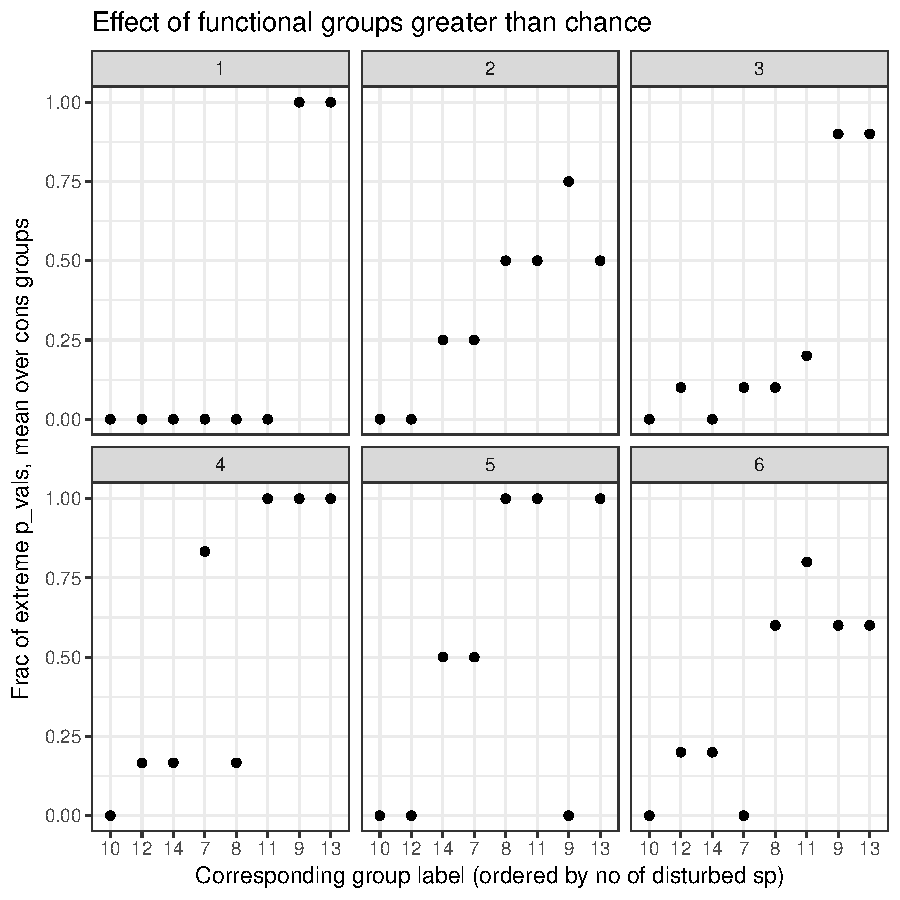
\includegraphics[width=1\textwidth]{../Results/Figures/A3B3/random/p_val.pdf}
  \caption{Effect of disturbing a number of randomly chosen basal species, corresponding to the size of the original trophically similar groups following Baskerville et al. \citep{Baskervilleetal2011}. The x-axis is ordered by the size of the corresponding group label, going from the smallest corresponding group number to the largest group. The y-axis shows the fraction of extreme p-values  ($0.05>p>0.95$) within each groups of consumer species (panels). If persistences for \emph{all} species included in a group of consumers are different ($0.05>p>0.95$) from what's expected by chance (random disturbance), the fraction of extreme p-values will be 1. If persistences of \emph{no} species in a specific consumer group is similar to what's expected by chance, the fraction of extreme p-values will be 0. The displayed value is a mean over all species included in each consumer group. Therefore, the fraction can vary from 0-1.}
  \label{fig:p_val}
\end{figure}

\begin{figure}[!p]
\centering
	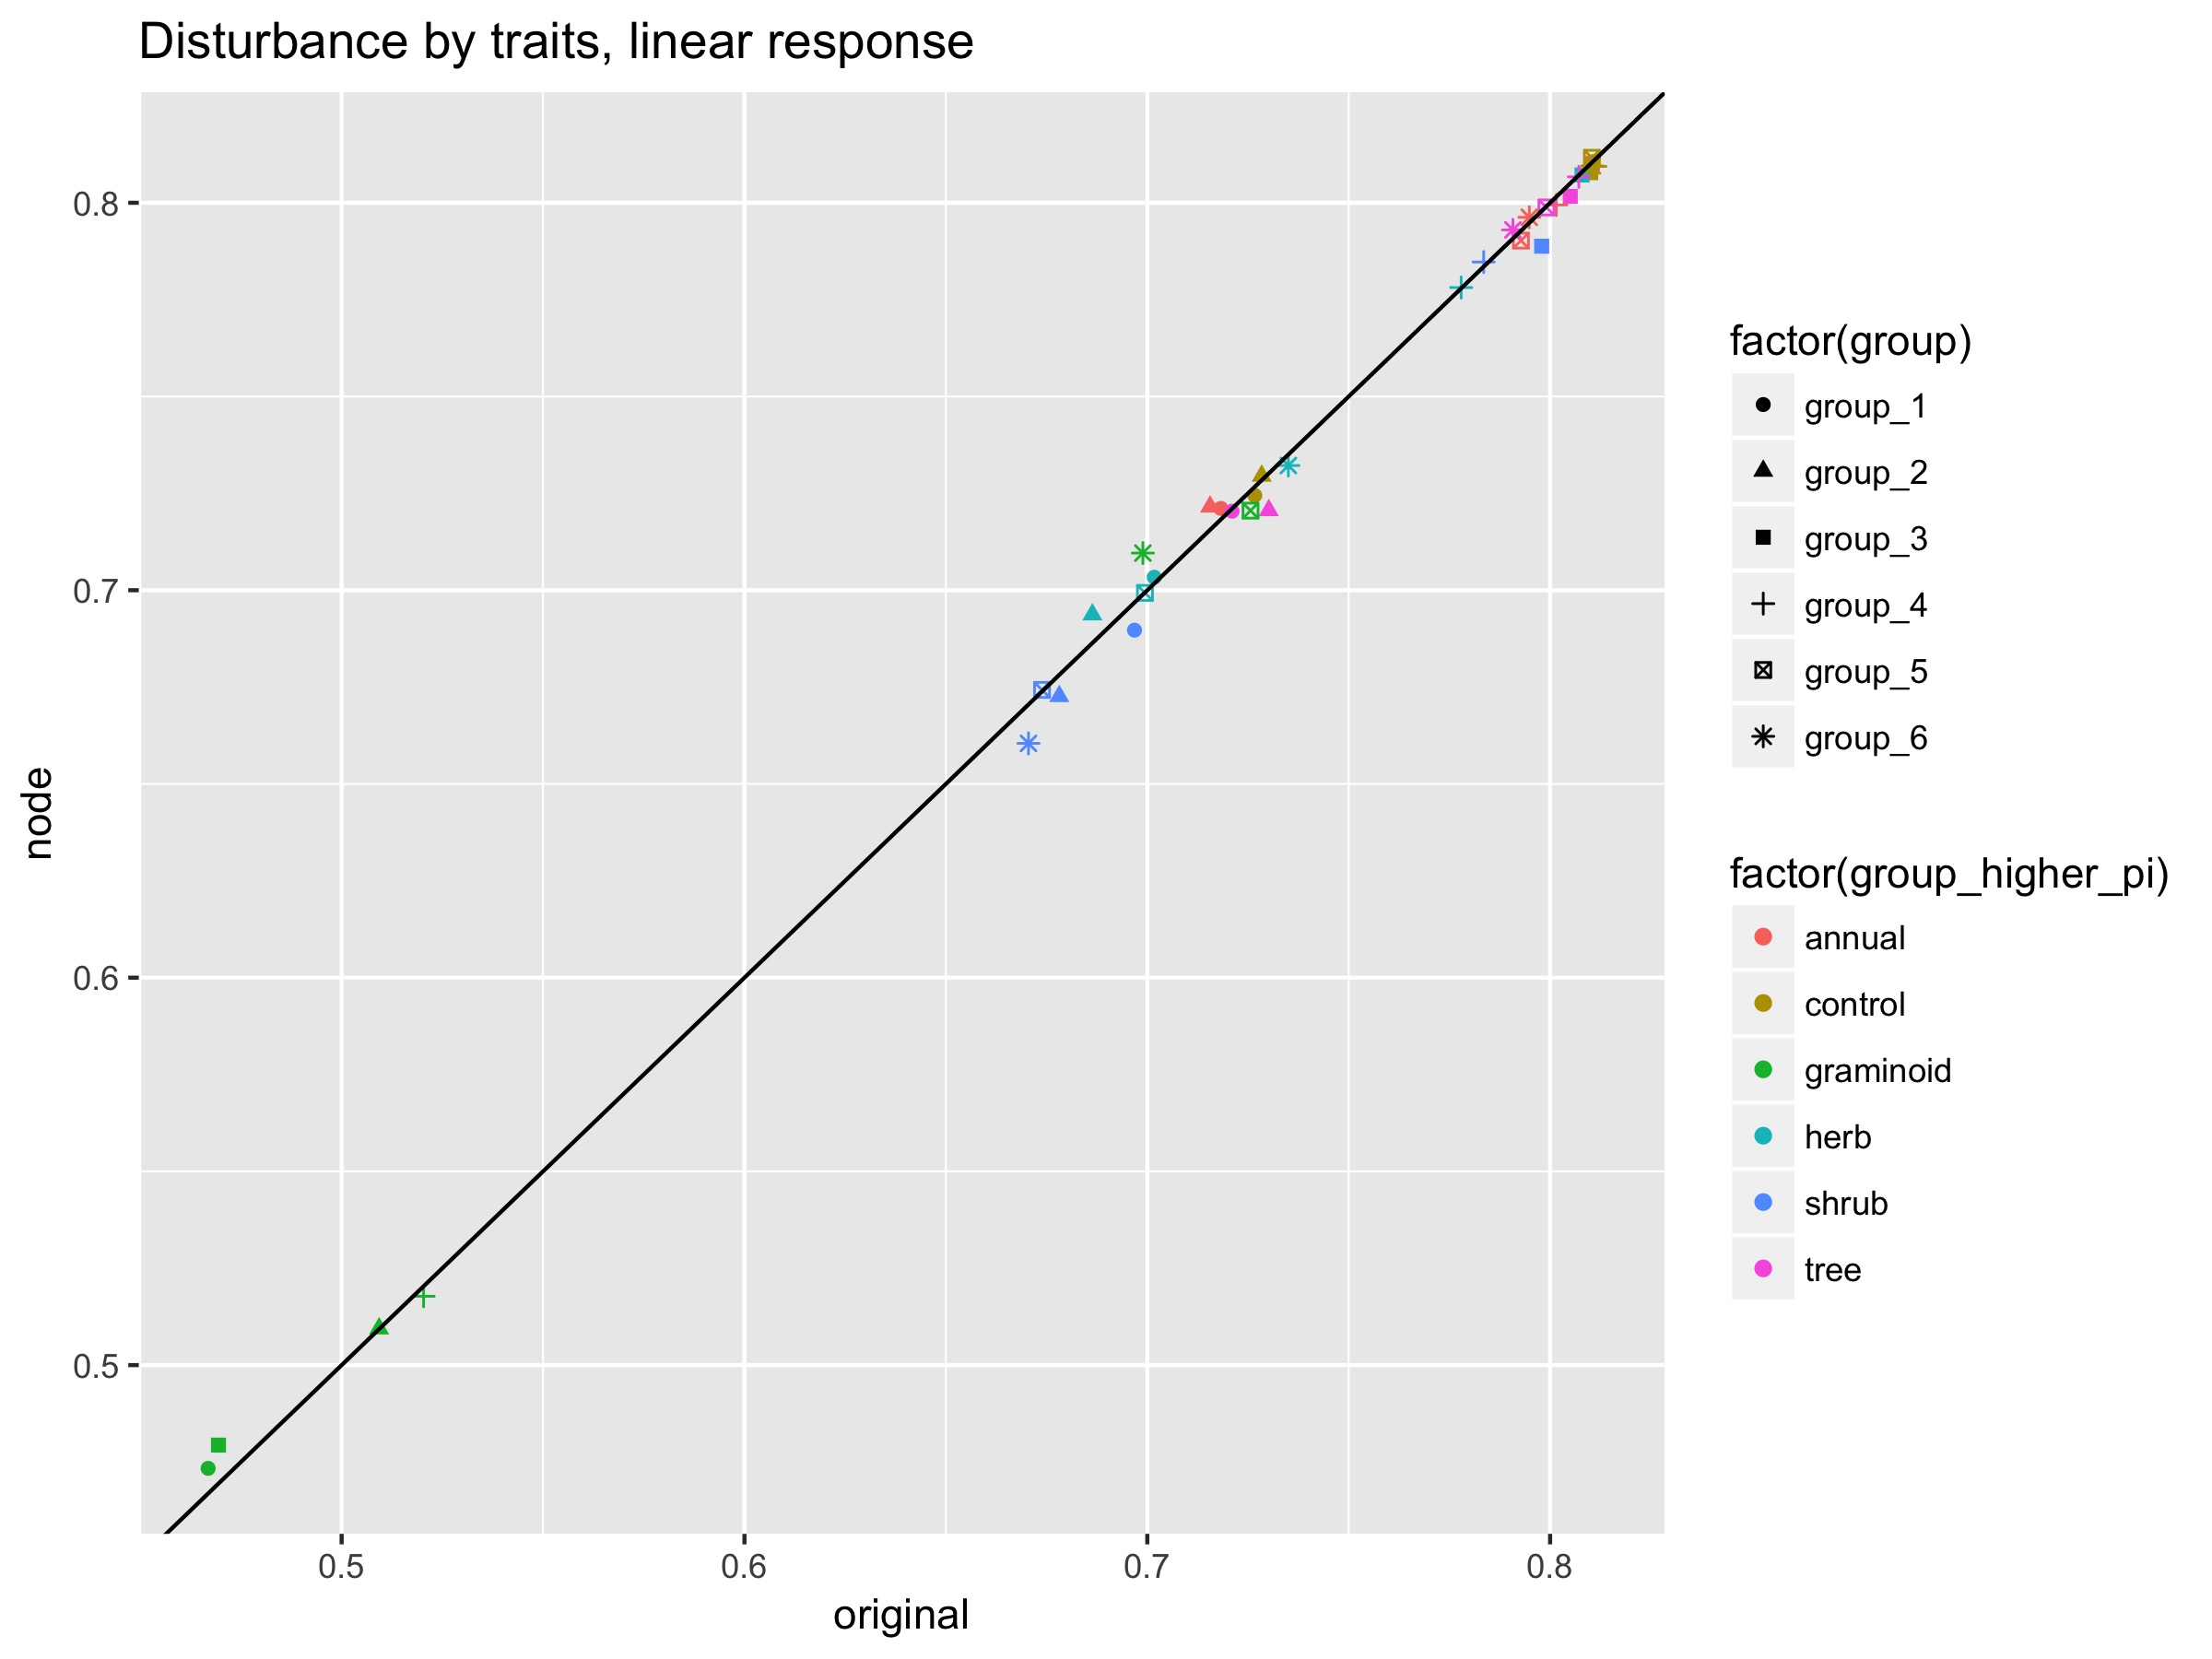
\includegraphics[width=0.49\textwidth]{../Results/Figures/Linear/comp_node_orig_traits.jpg}
	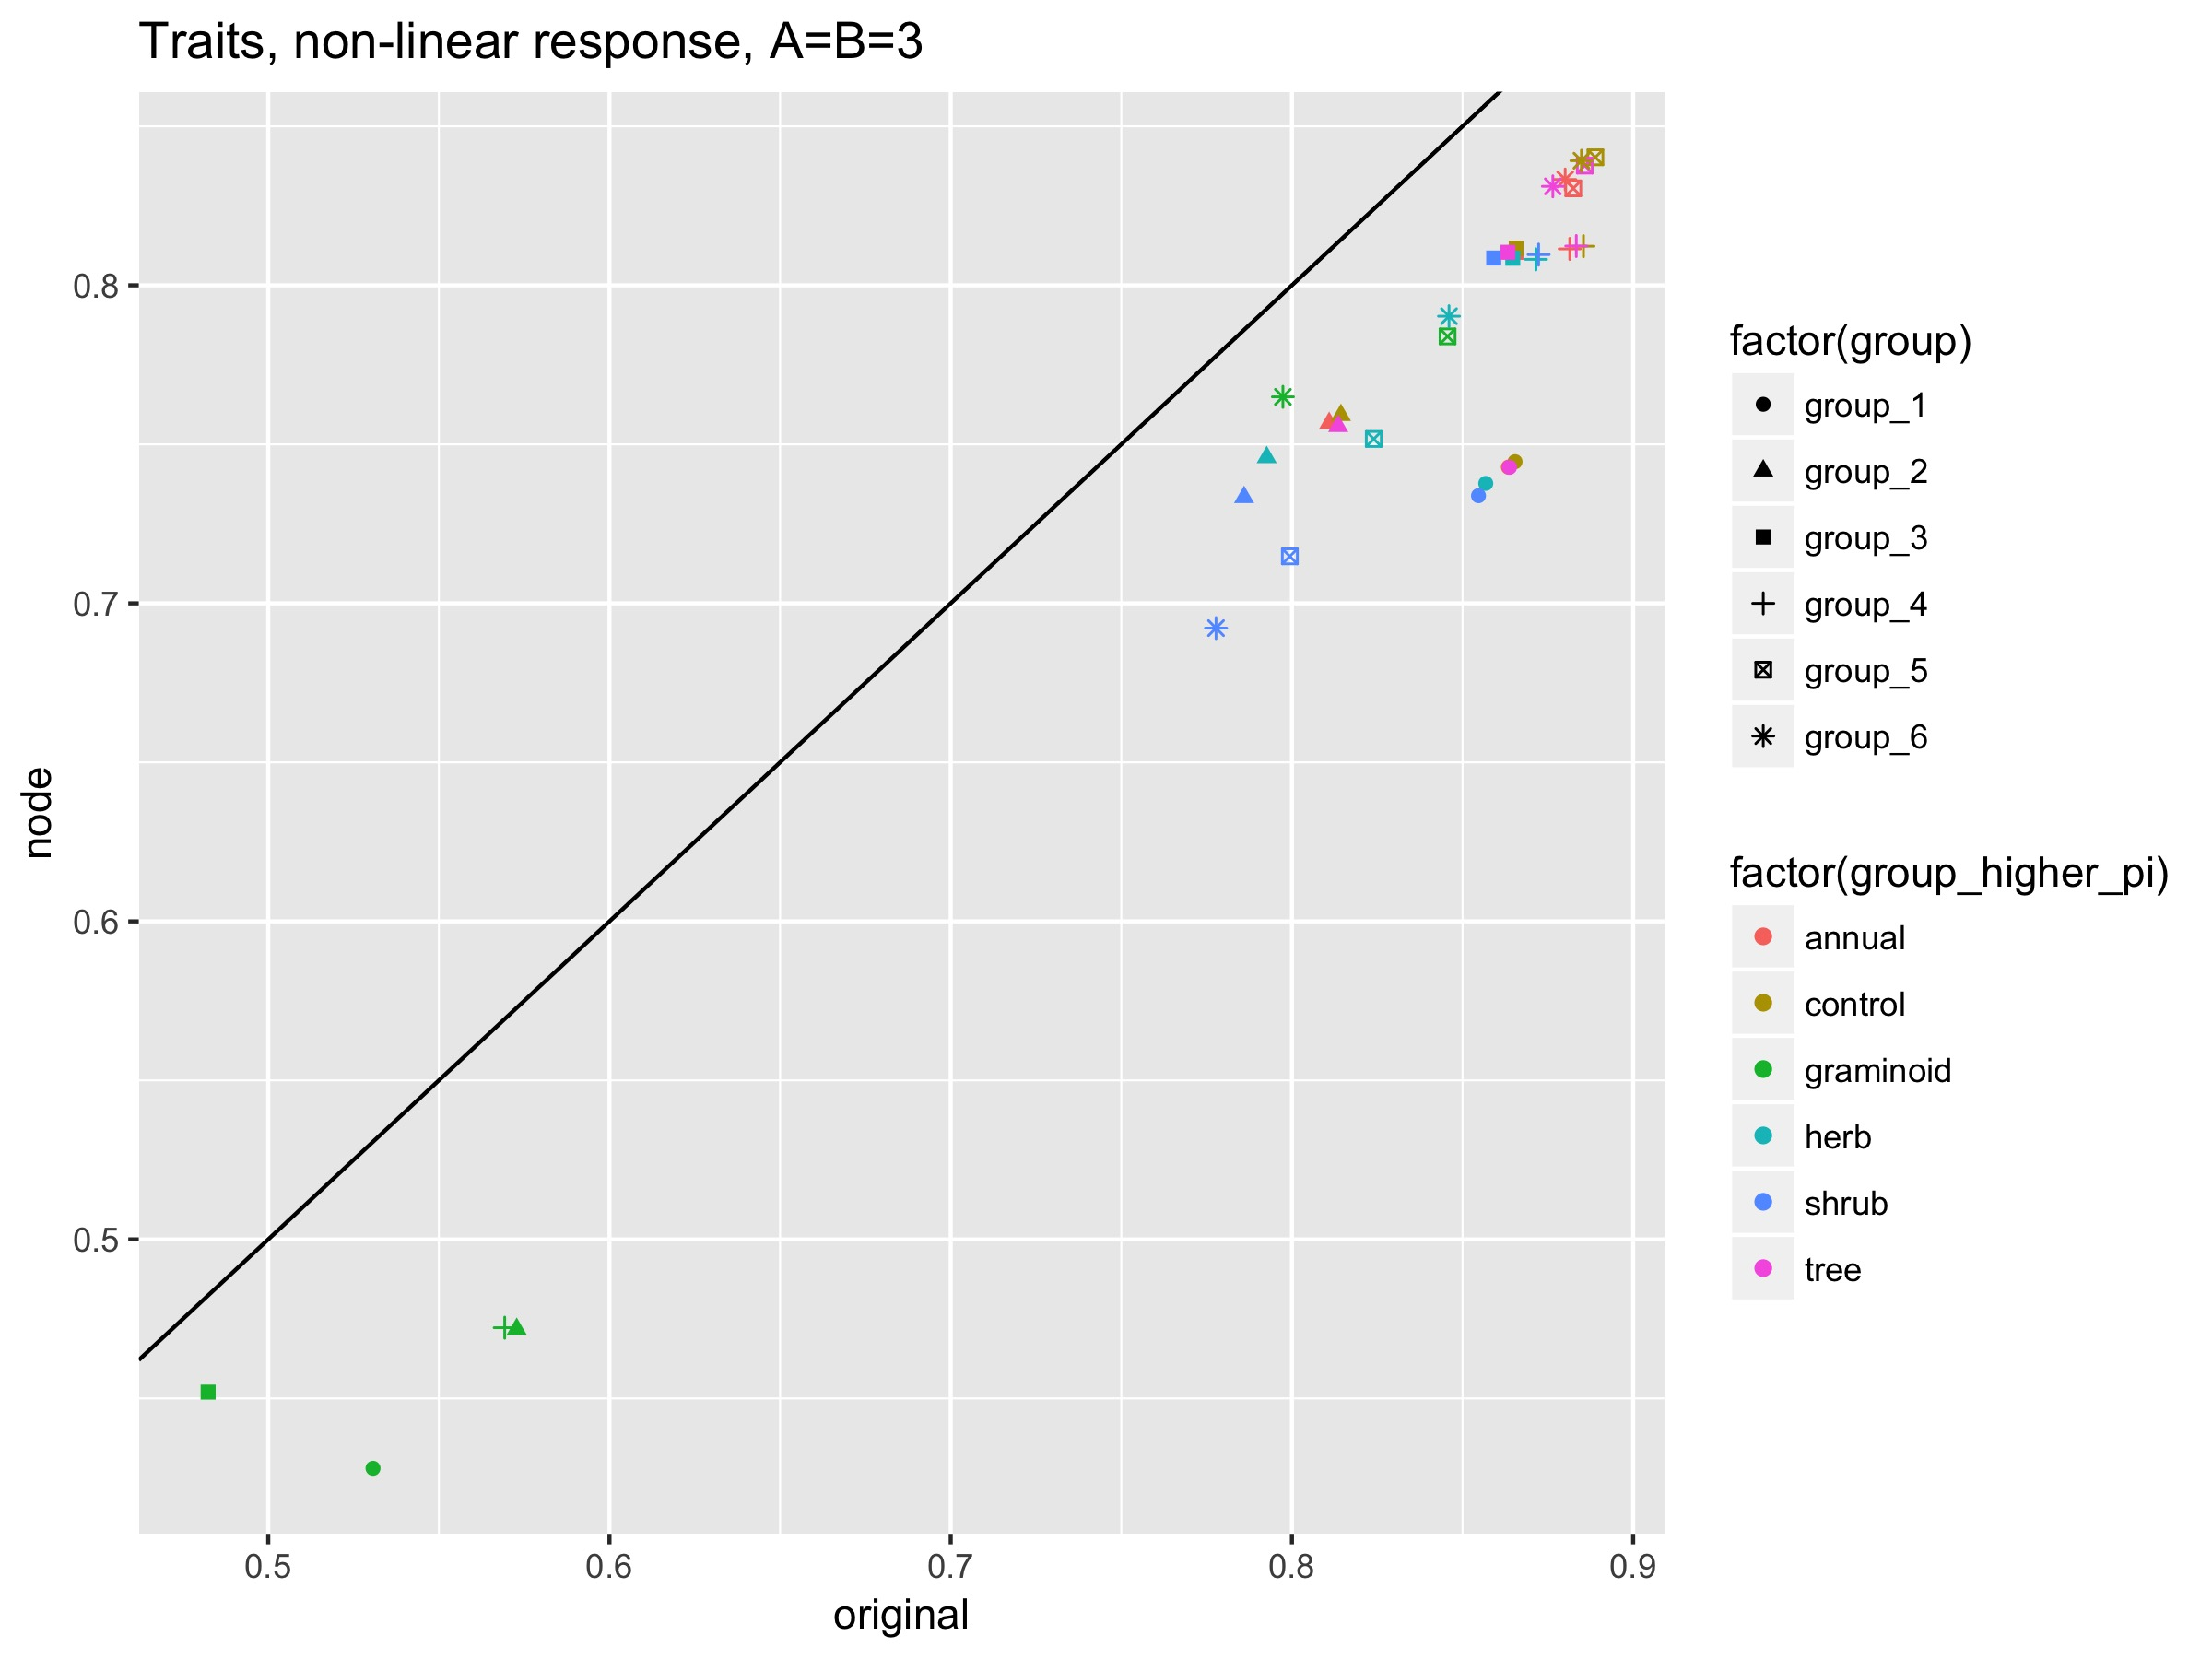
\includegraphics[width=0.49\textwidth]{../Results/Figures/A3B3/comp_node_orig_traits.jpg}
\caption{Comparison between persistence of consumer species in the original Serengeti network (x-axis) and the same network collapsed into nodes (y-axis). In the original network, a mean persistence for each group of consumers is presented. Symbols represent groups of consumer species, colors represent the trait character of plant species being disturbed. Values close to the diagonal show consistent values of persistence between the two types of network. Sub-figures show a) linear functional response ($alpha=beta=1$) to the loss of prey species, b) non-linear functional response ($alpha=beta=3$) to the loss of prey species.}
  \label{fig:collapsed_traits}
\end{figure}

\begin{figure}[!p]
\centering
	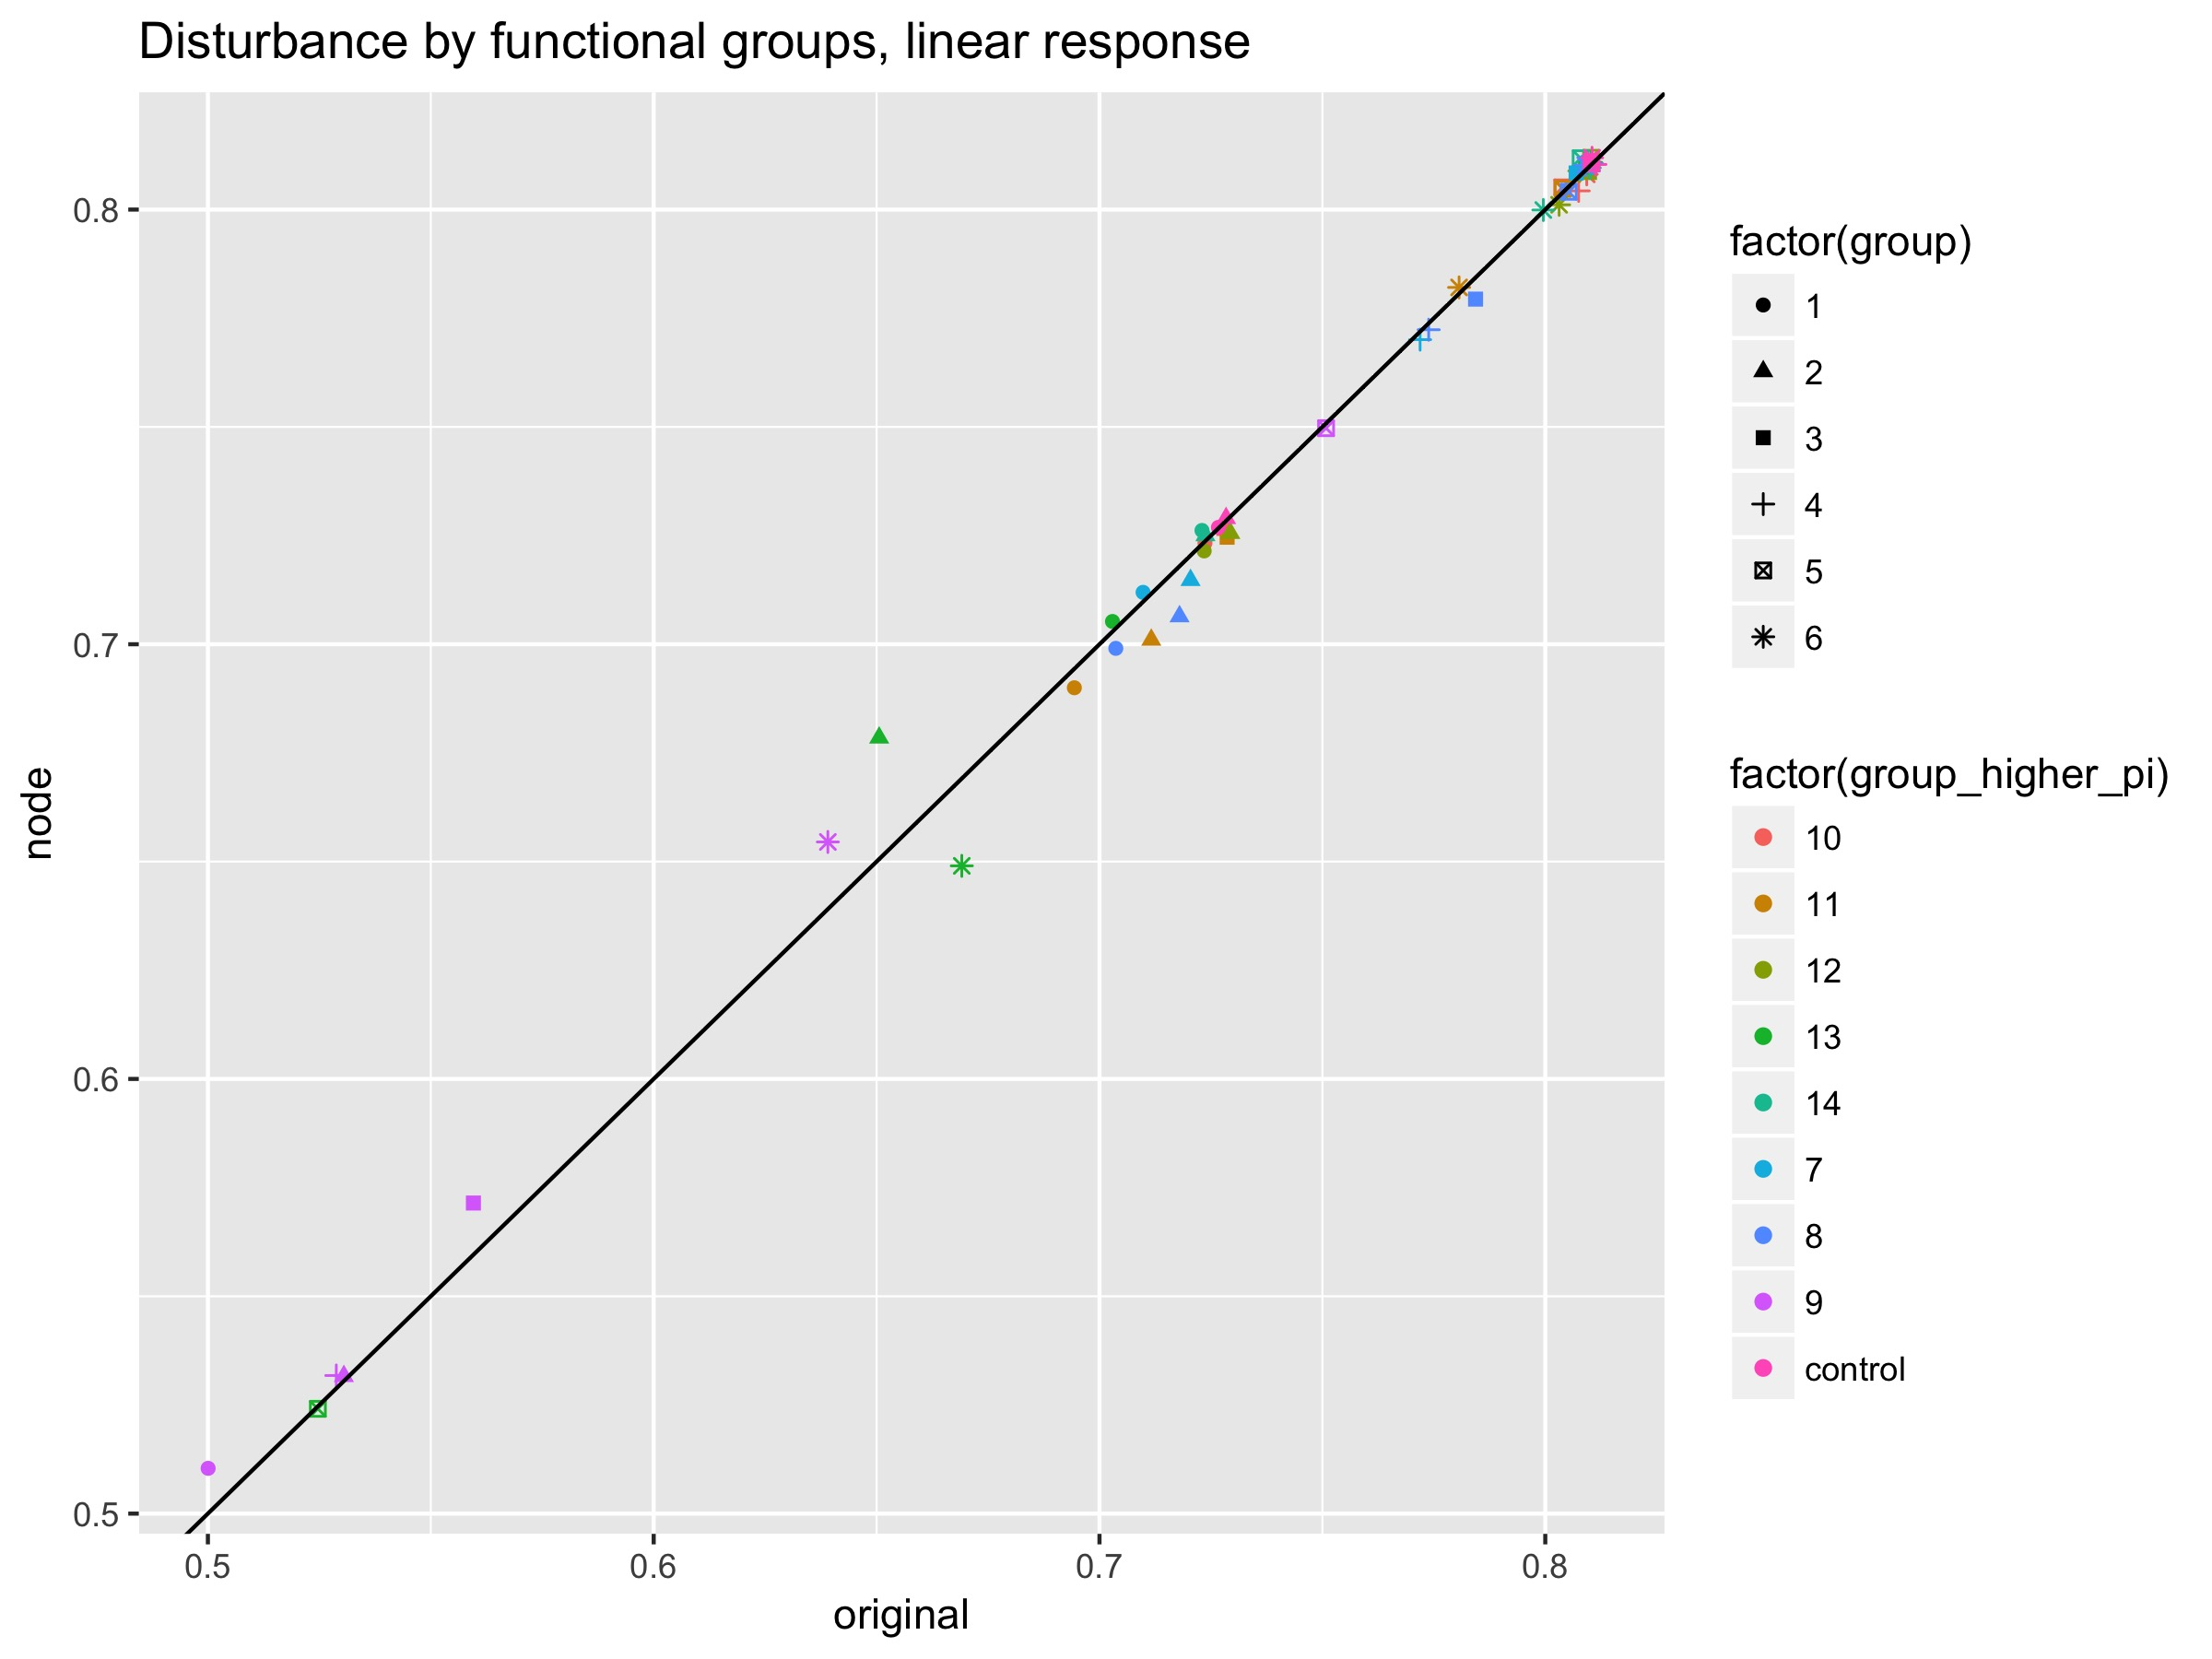
\includegraphics[width=0.49\textwidth]{../Results/Figures/Linear/comp_node_orig_groups.jpg}
	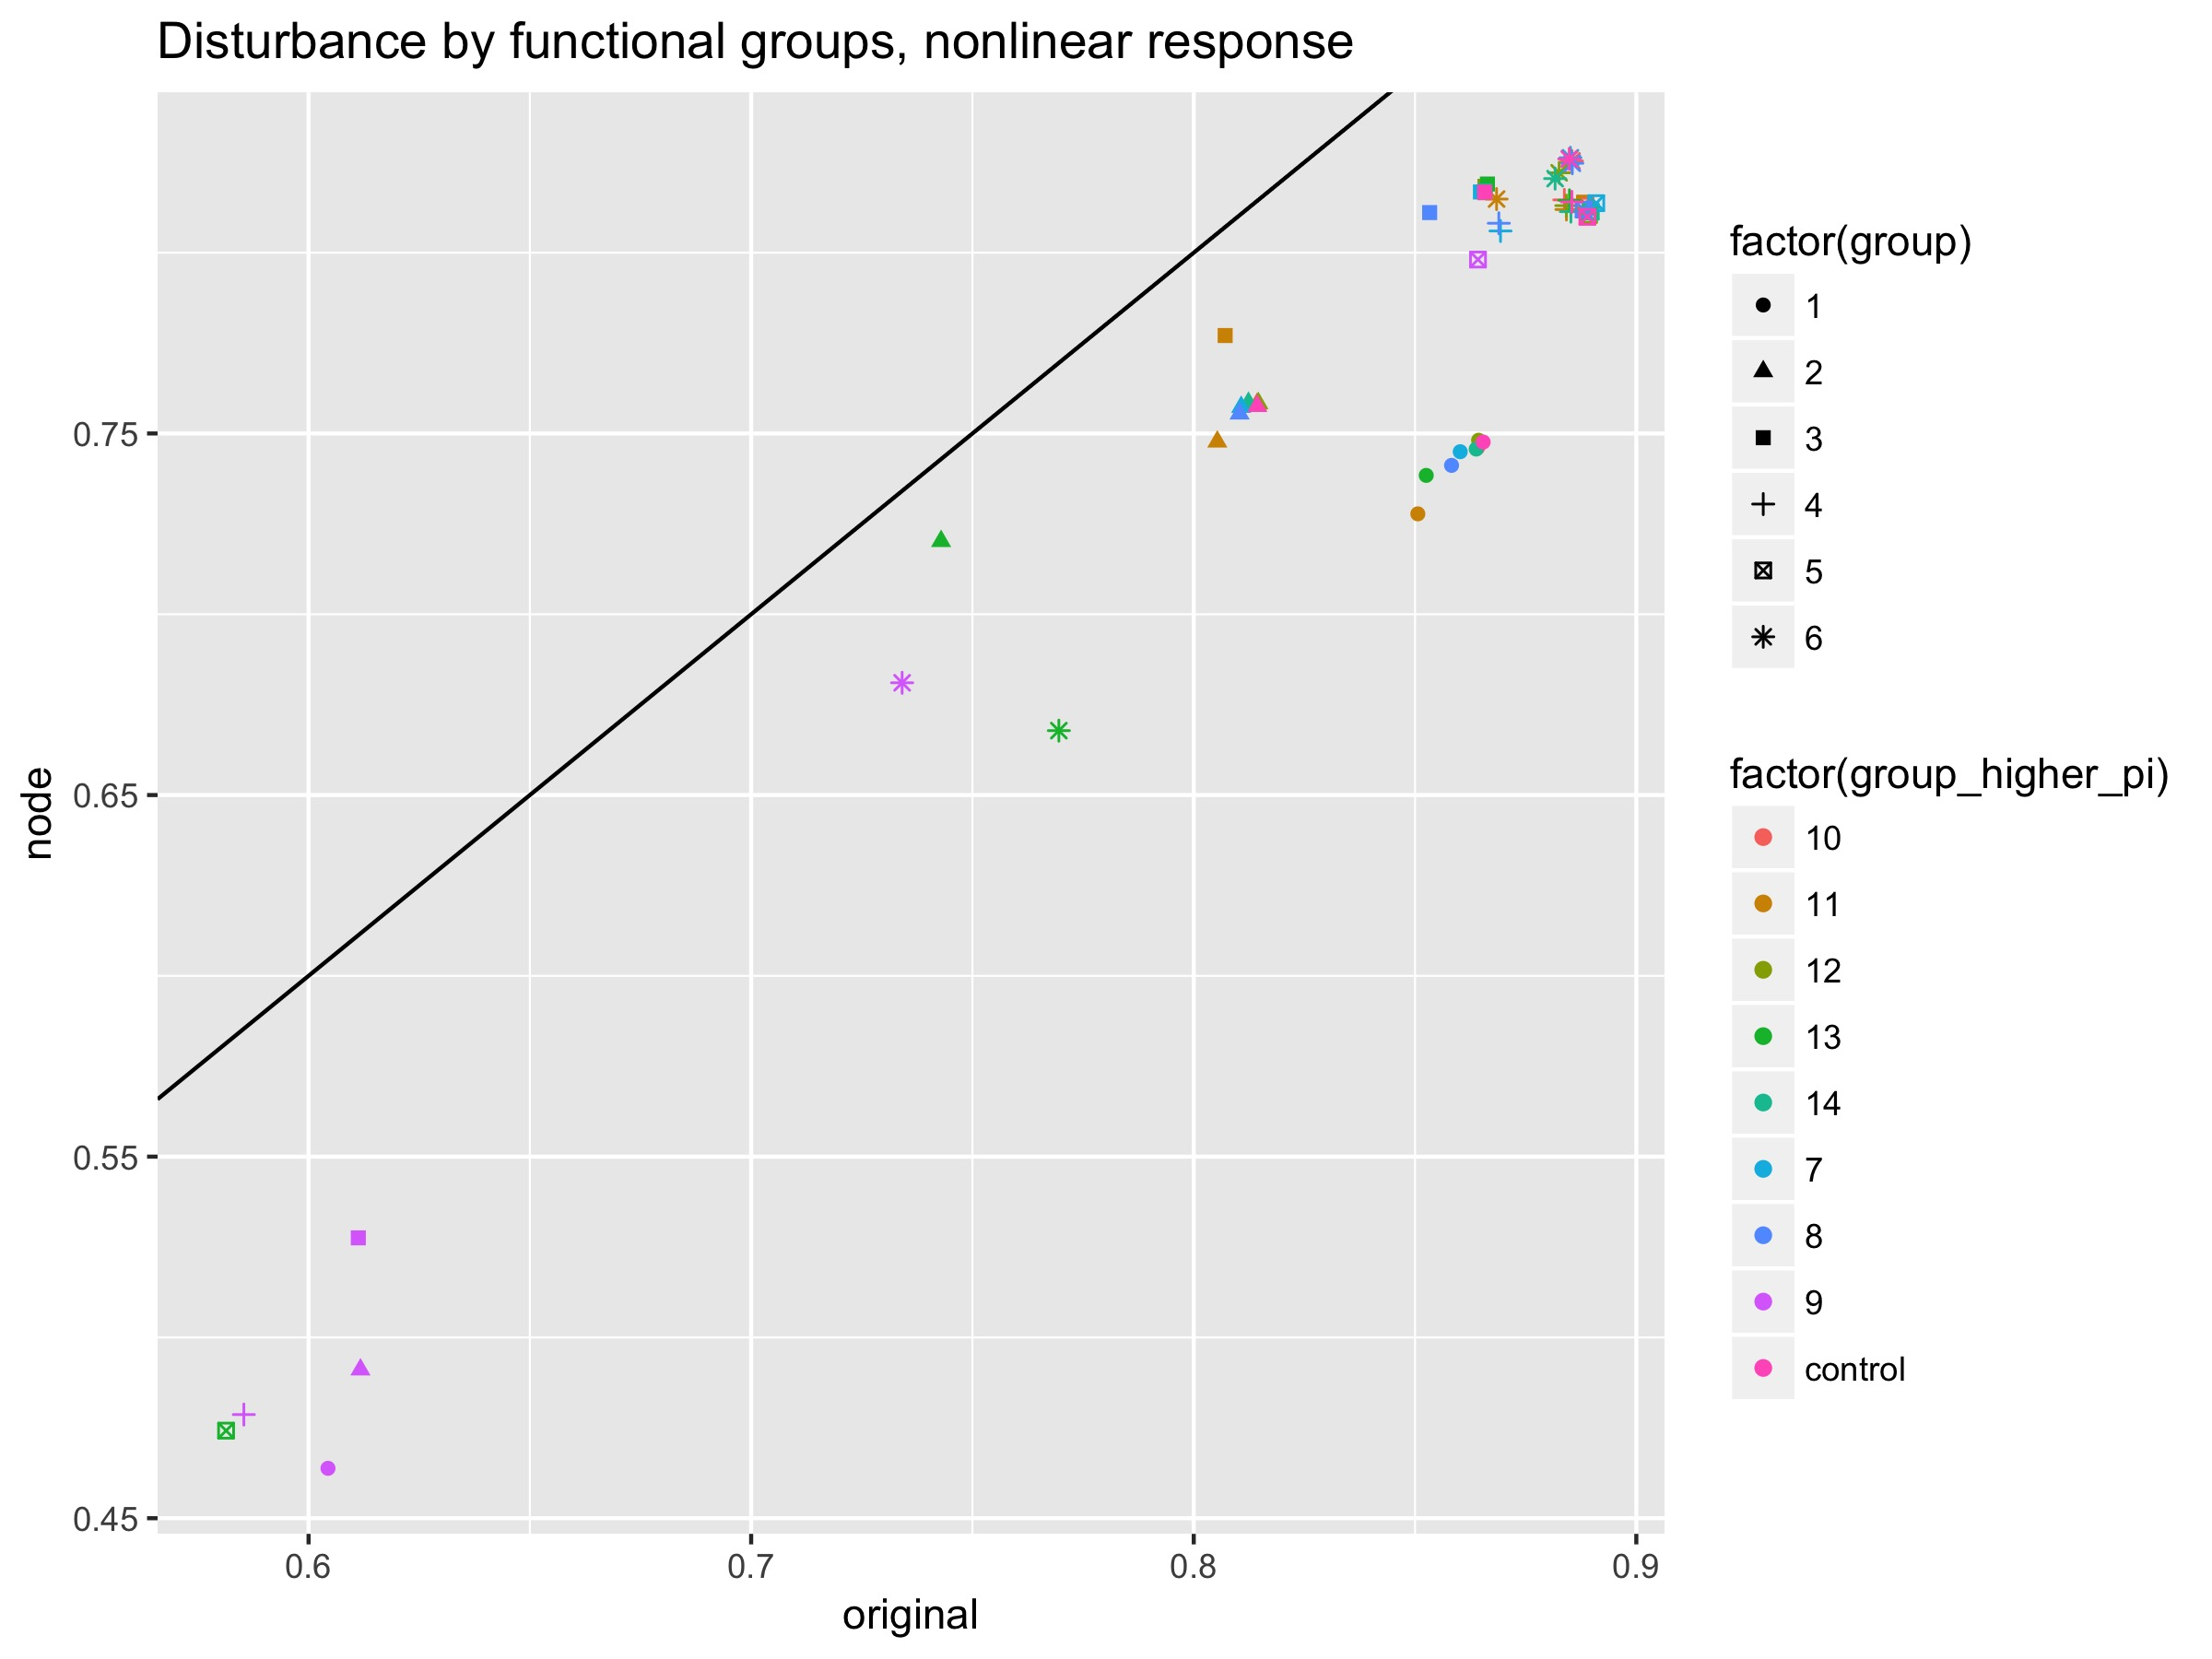
\includegraphics[width=0.49\textwidth]{../Results/Figures/A3B3/comp_node_orig_groups.jpg}
\caption{Comparison between persistence of consumer species in the original Serengeti network (x-axis) and the same network collapsed into nodes (y-axis). In the original network, a mean persistence for each group of consumers is presented. Symbols represent groups of consumer species, colors represent the trophically similar group of plant species being disturbed. Values close to the diagonal show consistent values of persistence between the two types of network. Sub-figures show a) linear functional response ($alpha=beta=1$) to the loss of prey species, b) non-linear functional response ($alpha=beta=3$) to the loss of prey species.}
  \label{fig:collapsed_groups}
\end{figure}

\begin{figure}[!p]
\centering
	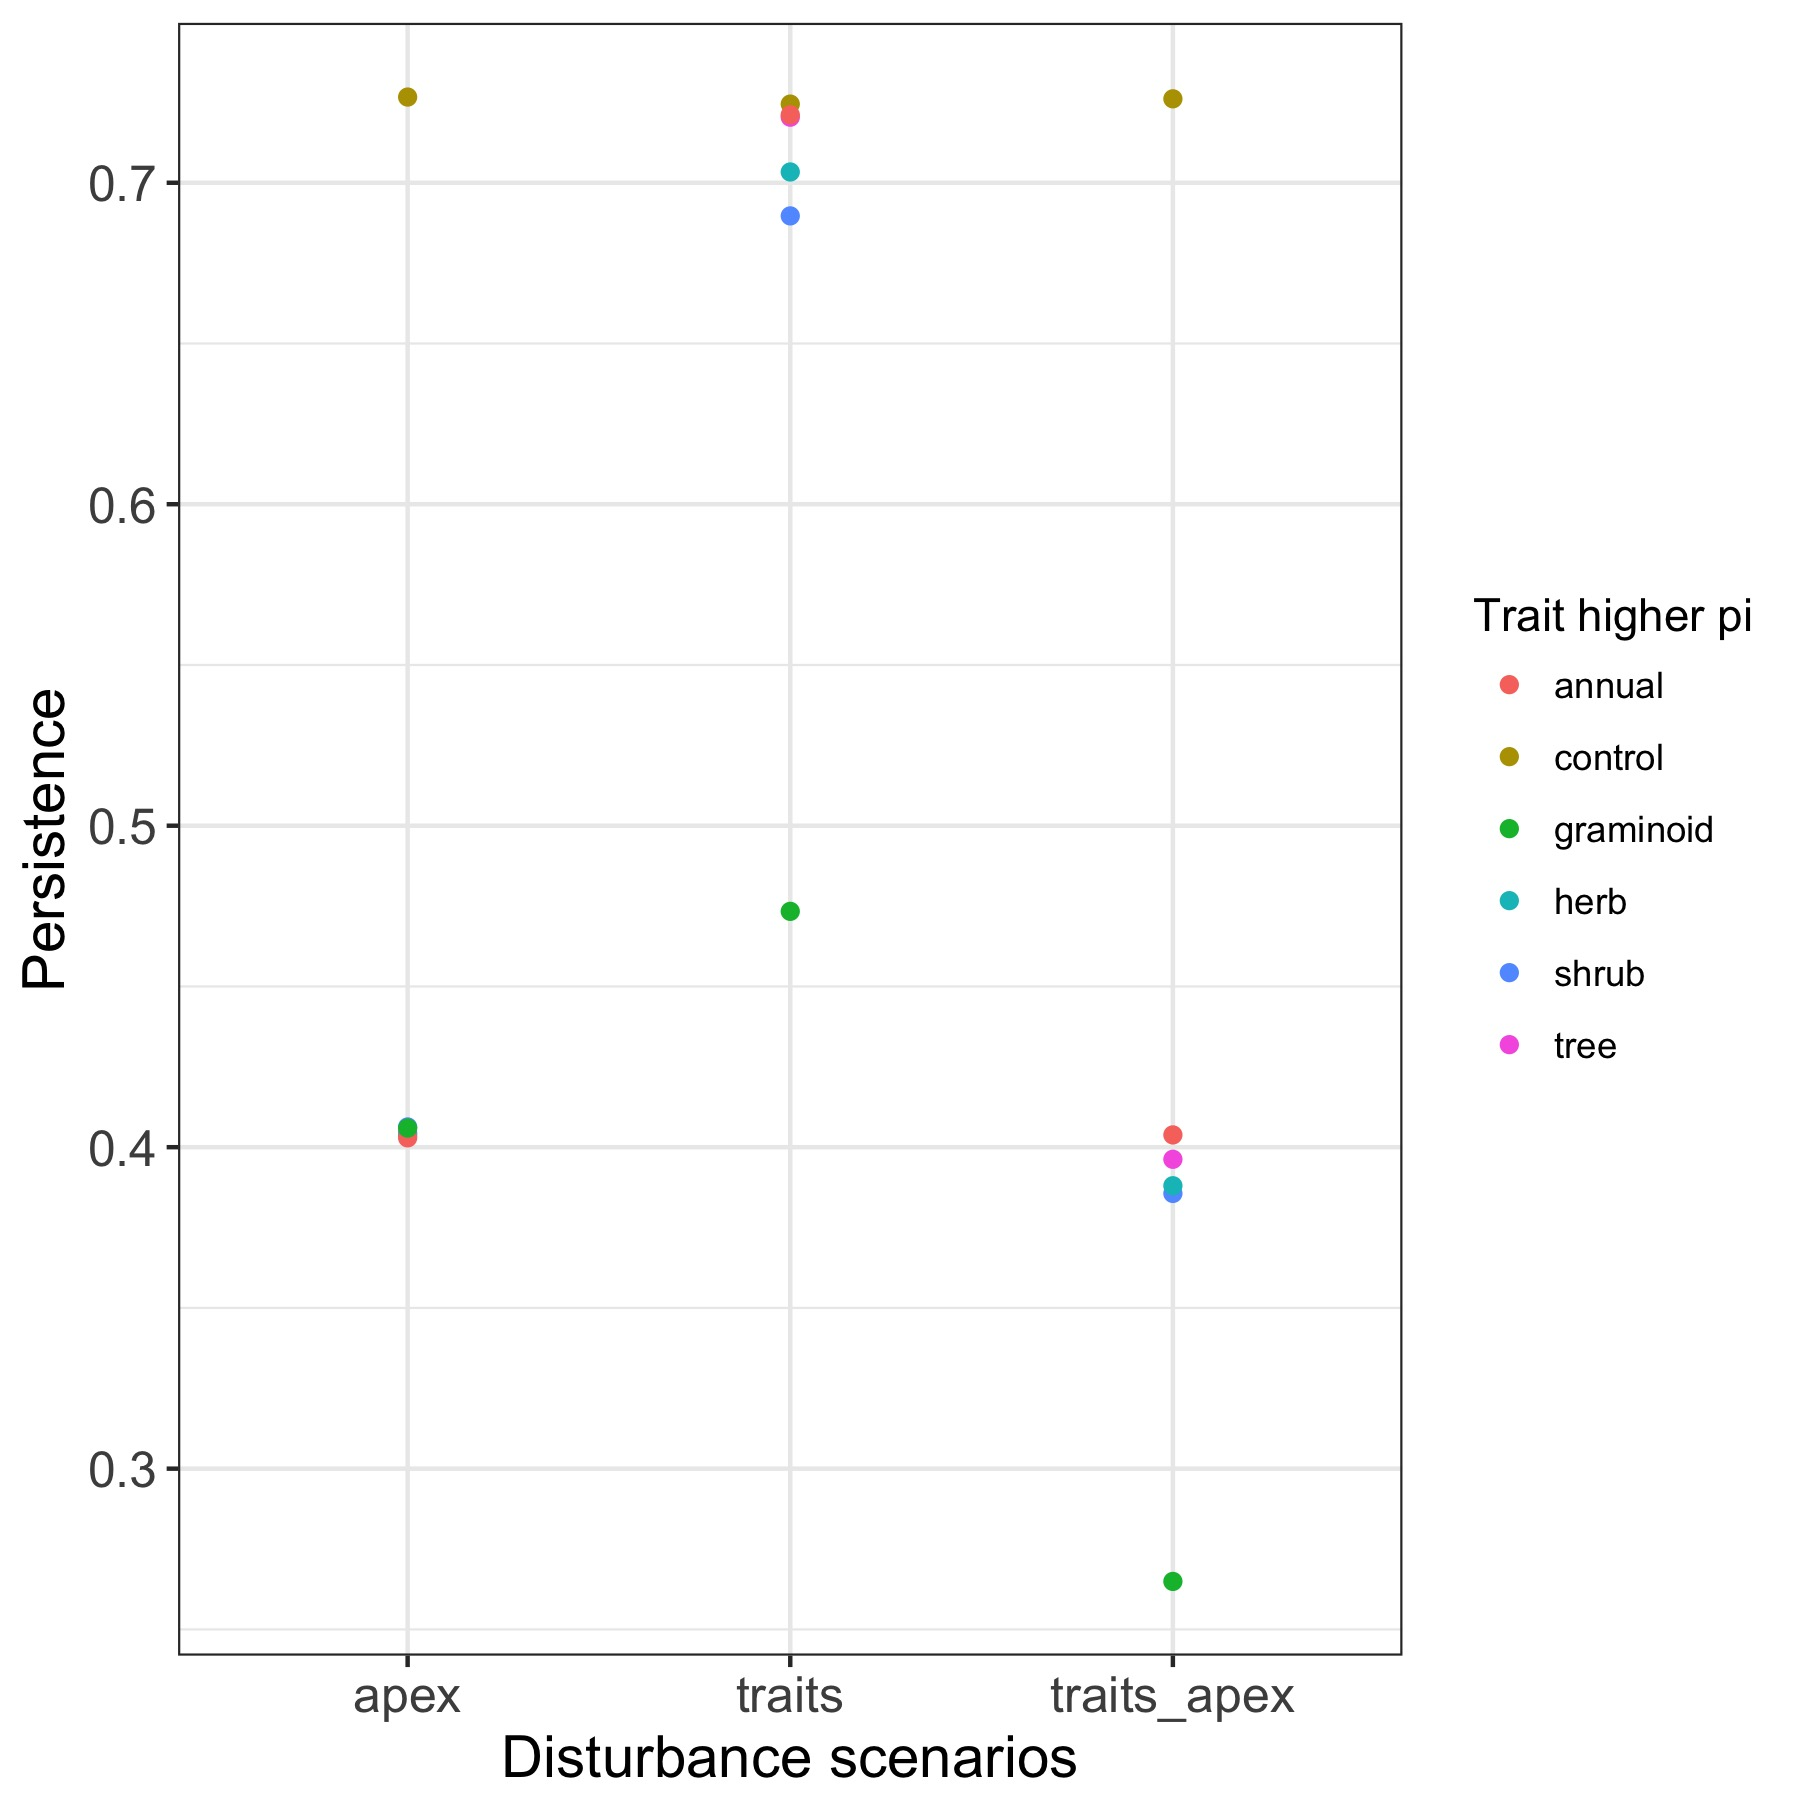
\includegraphics[width=0.47\textwidth]{../Results/Figures/Linear/collapsed_trait_apex.jpg}
	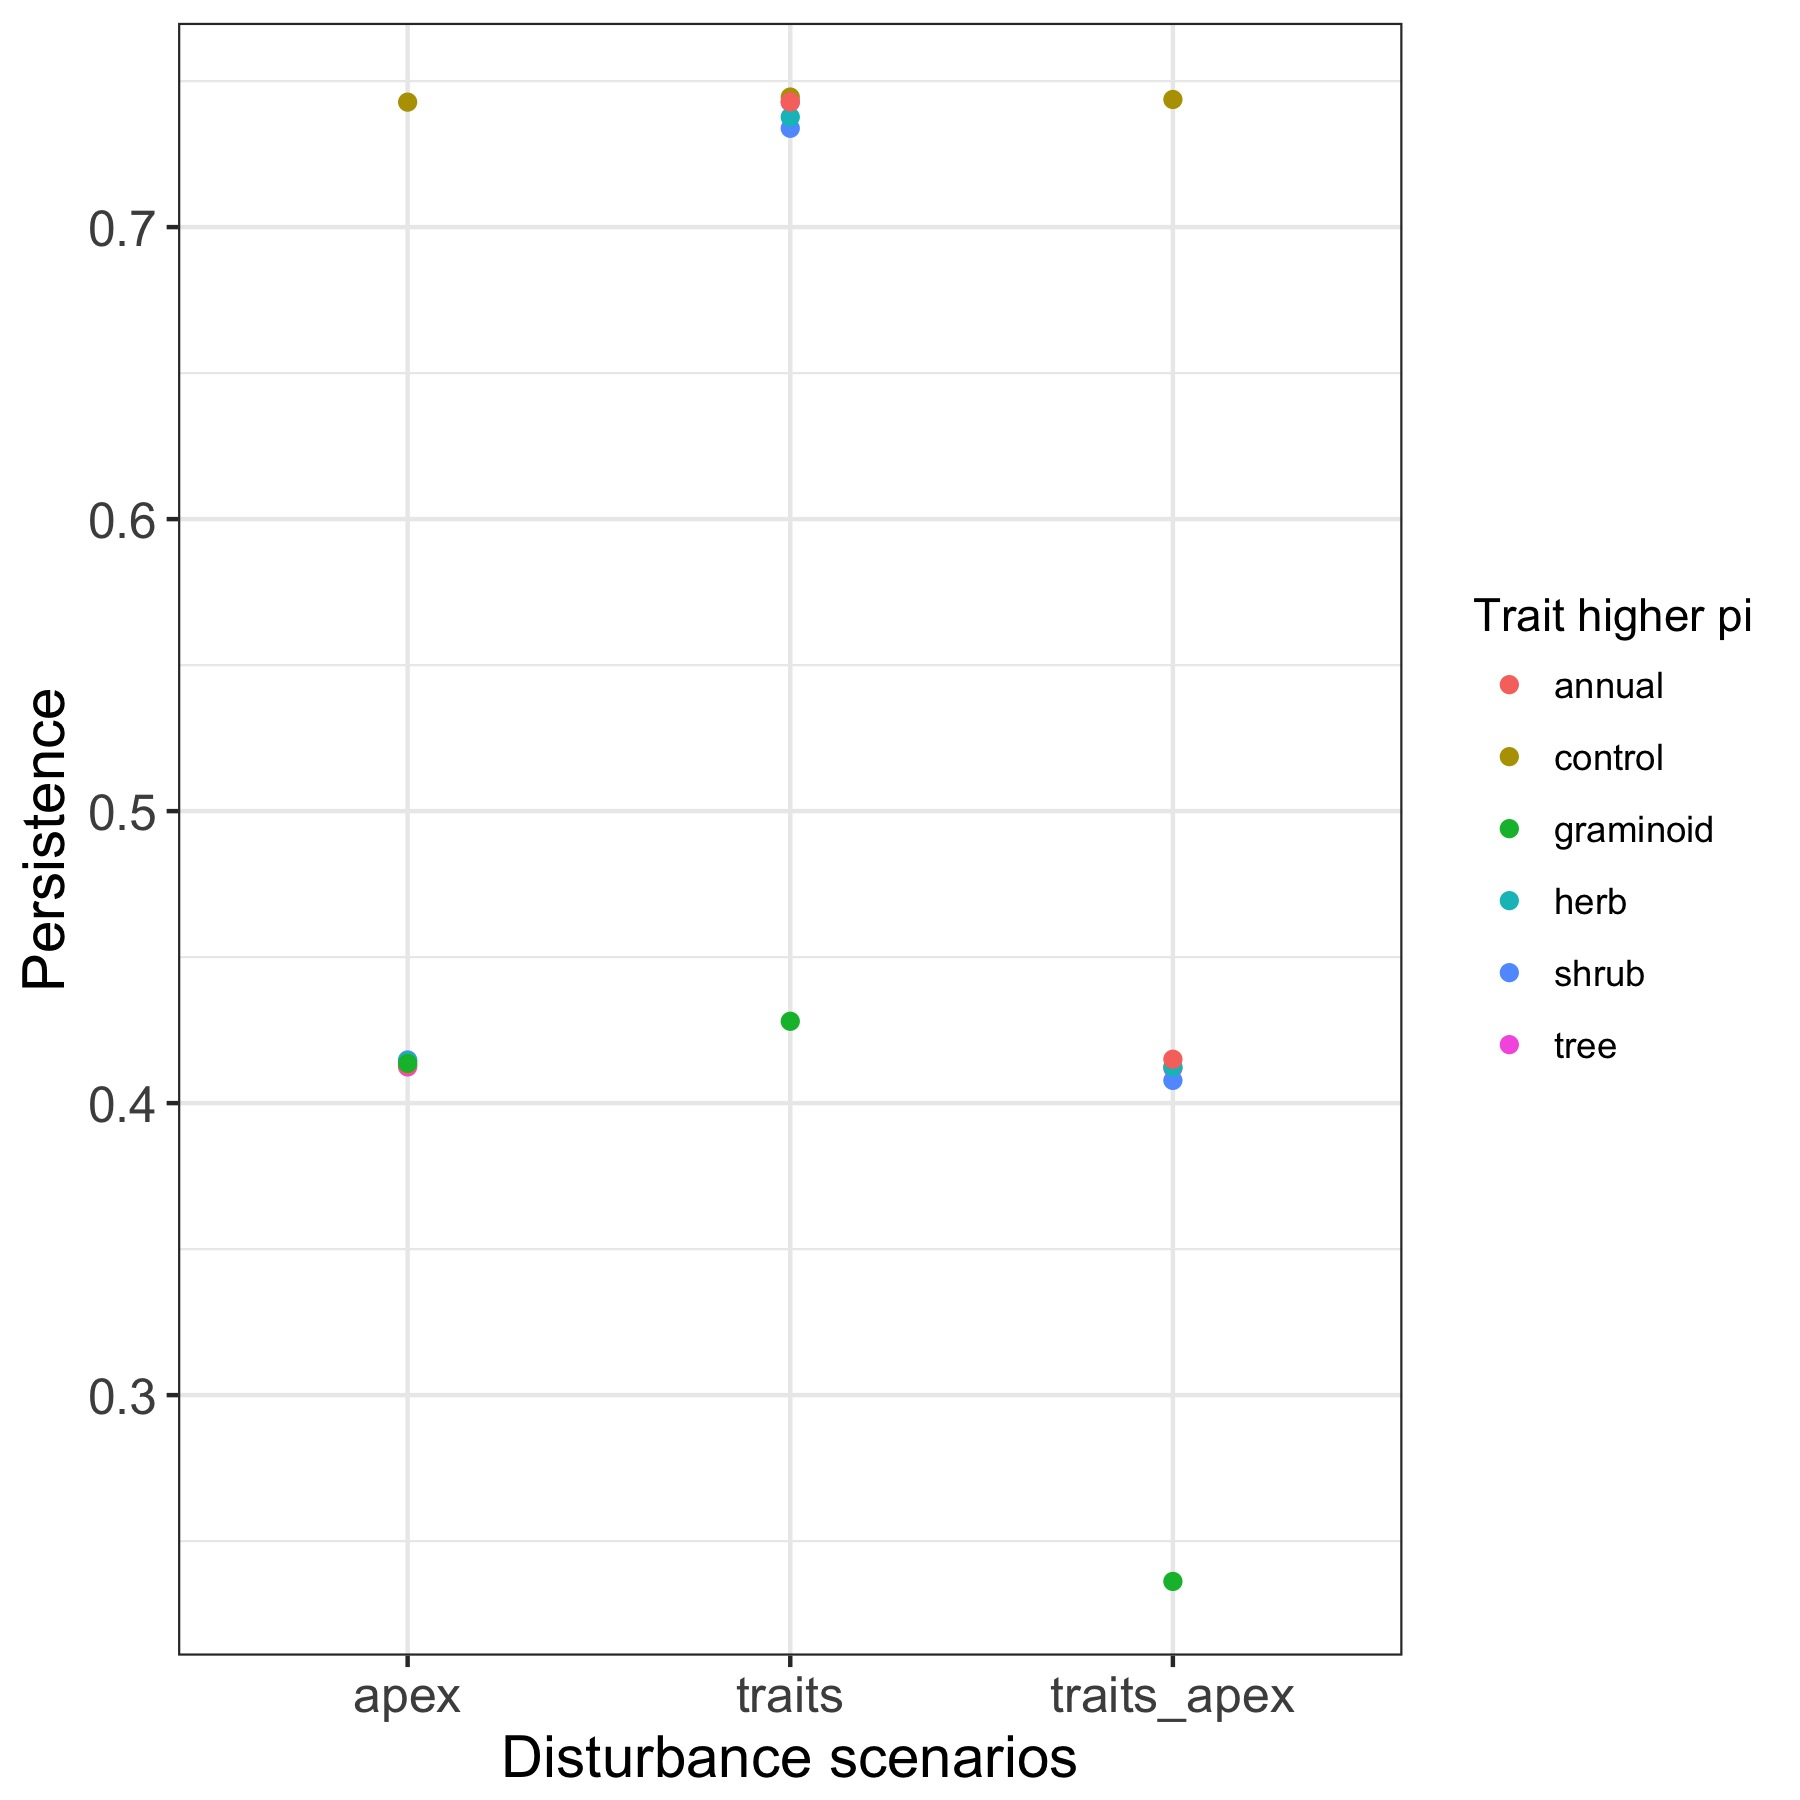
\includegraphics[width=0.47\textwidth]{../Results/Figures/A3B3/collapsed_trait_apex.jpg}
\caption{Persistence (y-axis) of apex predators in different disturbance scenarios (x-axis); a higher baseline probability for only apex predators (apex), a higher baseline probability for various plant traits (see legend, traits), a higher baseline probability for various plant traits (see legend) and for apex predators (traits apex). Sub-figures show a) linear functional response ($alpha=beta=1$) to the loss of prey species, b) non-linear functional response ($alpha=beta=3$) to the loss of prey species.}
  \label{fig:apex_trait}
\end{figure}

\clearpage			% clears the page - whatever comes next starts off on a new page


\bibliographystyle{unsrt}
\bibliography{bib_serengeti}


\end{document}
